% !TeX program = lualatex
\documentclass{jit-qut}

\newcommand{\guideversion}{V26.1.6.1}

\title{\zihao{-2}\bfseries JIT-QUT 项目求生指南\\[0.35em]{\zihao{-4}\mdseries\texttt{\guideversion}}}
\author{李京儒~缪彭哲}
\date{2026 年 9 月}

\setcounter{tocdepth}{2}

\begin{document}

\maketitle
\section*{前言}
\addcontentsline{toc}{section}{前言}

这本《JIT--QUT 项目求生指南》写给正在了解, 准备参加或已经进入金陵科技学院与昆士兰科技大学（QUT）合作项目的同学. 我们希望把项目中的课程安排, 升学衔接, 语言要求, 费用预算, 住宿选择以及 QUT 生活等信息整理在一起, 让大家能够更快建立对整个项目的认识, 也少走一些可以避免的弯路.

本指南不是学校的正式通知, 也不能替代学校, QUT 或 QUT College 发布的最新文件. 文中的课程, 学费, 开课安排, 语言要求, 校历和住宿信息均可能随时间调整; 阅读时请结合个人的录取结果, Advanced Standing, Study Plan 以及学校的最新通知进行判断. 对于重要事项, 请始终以相关官方页面和正式文件为准.

内容编排上, 前半部分主要帮助读者了解项目和每学期课程, 后半部分补充语言准备, 费用估算, 学术日历, 校园地图和住宿房型等资料. 附录中的地图与日历尽量保留原始版式, 方便查阅和保存.

这份指南会随着项目和资料的变化持续修订. 后续你们的先驱者也会持续更新. 本指南的代码库已上传至 \official{https://github.com/Leamon-Lee/jit-qut-undergraduate-guidebook}{GitHub 代码库}, 欢迎通过提交或反馈共同完善内容.

本指南采用 \texttt{VYY.R.D.C} 的版本号规则. 当前版本号为 \texttt{\guideversion}\footnote{版本号中的 \texttt{YY} 为编写年份, \texttt{R} 为该年度的公开版本序号, \texttt{D} 为该版本的编写修订次数, \texttt{C} 为已确认的学长学姐人数. 例如, \texttt{V26.5.1.1} 表示 2026 年第 5 个公开版本的第 1 次编写修订, 并有 1 位学长学姐确认; 是否达到“广泛确认”应以实际确认范围为准.}.

本项目采用 MIT License\footnote{MIT License 适用于本仓库中的原创文字, LaTeX 代码, 排版结构和原创素材, 允许查看, 编辑, 复制, 再发布和商业使用, 但必须保留版权声明和许可证文本. 仓库中的部分图片, PDF, 地图, 字体和代码属于第三方材料, 其版权和许可仍归原权利人所有, 使用时应遵守相应来源的要求. 完整条款见仓库中的 \official{https://github.com/Leamon-Lee/jit-qut-undergraduate-guidebook/blob/master/LICENSE}{MIT License 文件}}.

如果你发现内容已经过时, 或者有更准确的官方信息, 欢迎以最新文件为依据进行补充和更正. 希望它能成为一份实用, 诚实而且真正帮得上忙的项目手册.

\clearpage
\tableofcontents

\clearpage
\section{先了解这个项目}

本指南所介绍的项目原先由国际教育学院负责, 自2026年开始纳入软件工程学院. 原先的项目背景可以查看 \official{https://iec.jit.edu.cn/info/1126/1838.htm}{学校官方介绍}. 但是作为过来人, 里面的相关信息可能没有及时更新, 具体要以学校的实际安排为准. 同时, 该项目已被教育部中外合作办学监管工作信息平台收录, 可查看项目的\official{https://www.crs.jsj.edu.cn/aproval/detail/648}{审批信息}. 

\subsection{快速了解一下 QUT}
QUT 全称: \official{https://qut.edu.au/home}{昆士兰科技大学 (Queensland University of Technology)}. 学校位于昆士兰州的布里斯班, 布里斯班是昆士兰州的首府, 众所周知该城市将在 \official{https://www.olympics.com/zh/olympic-games/brisbane-2032}{2032 年举办夏季奥运会}. 截至本指南更新日 (2026 年 9 月), QUT 在最新的 QS World University Rankings 2027 中位列全球第 240 名; QS 2026 榜单中为第 226 名. 排名会随年度方法和数据更新, 只能作为学校整体的参考, 不能替代对具体专业, 课程和项目要求的判断. 排名数据可在\official{https://www.topuniversities.com/universities/queensland-university-technology-qut}{QS 官方 QUT 页面}核对.

\begin{figure}[H]
	\centering
	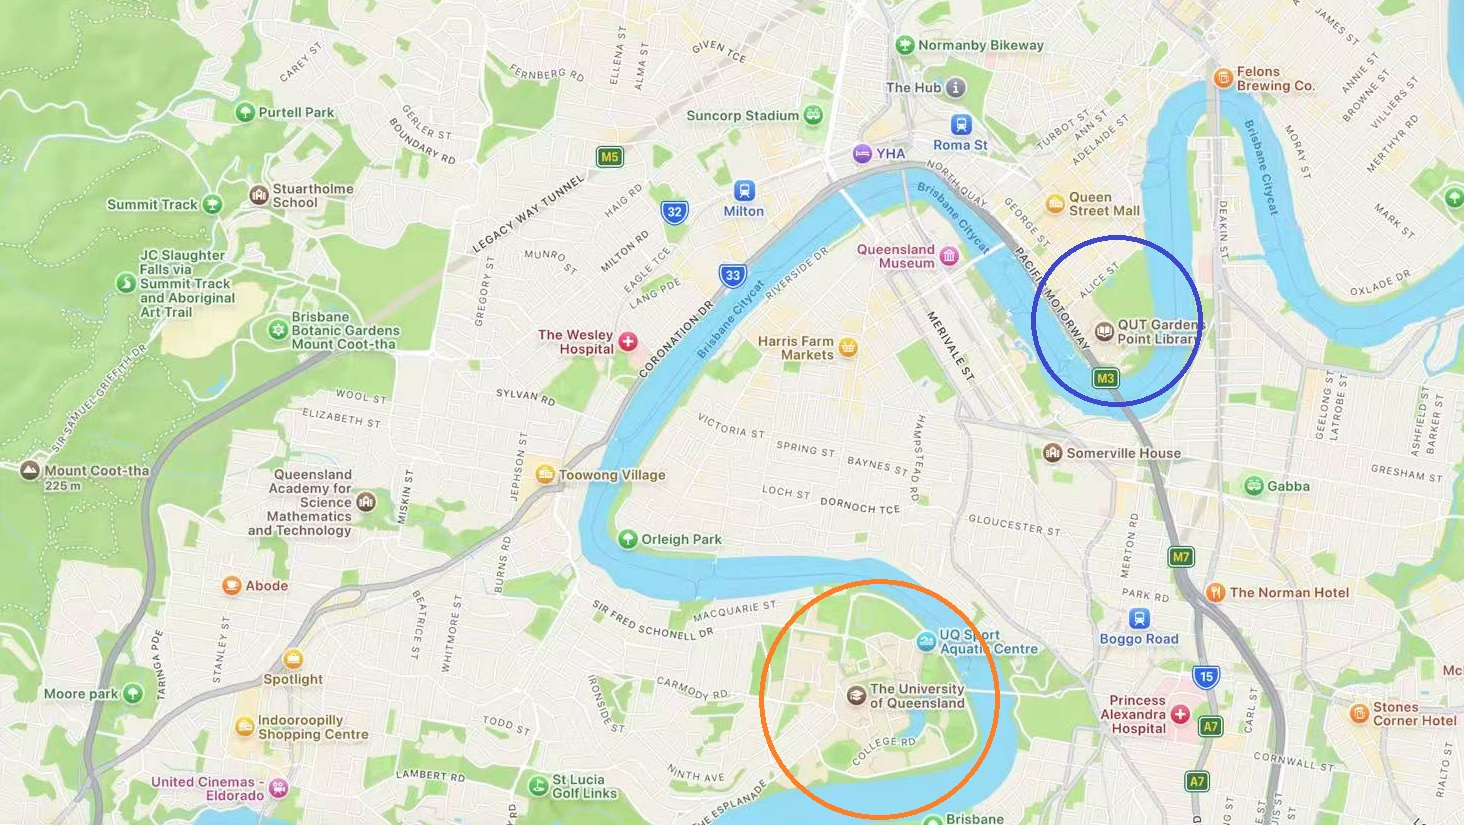
\includegraphics[width=0.8\textwidth,keepaspectratio]{pics/qut&uq-map.jpg}
\caption{QUT (蓝色圈) 和 UQ (橙色圈) 在布里斯班的位置}
\end{figure}


昆士兰州简称昆州, QUT 位于布里斯班的 Gardens Point (G.P.) 校区, 布里斯班也常被称为``布村''. QUT 与 UQ (昆士兰大学) 的校园地理位置较近, 相关地理信息见附录~\ref{app:geography}.

QUT分为两个校区, 而我们第四年所要去的是 G.P. 校区. 详细地理信息见附录 ~\ref{app:QUT-map}.

\begin{figure}[H]
	\centering
	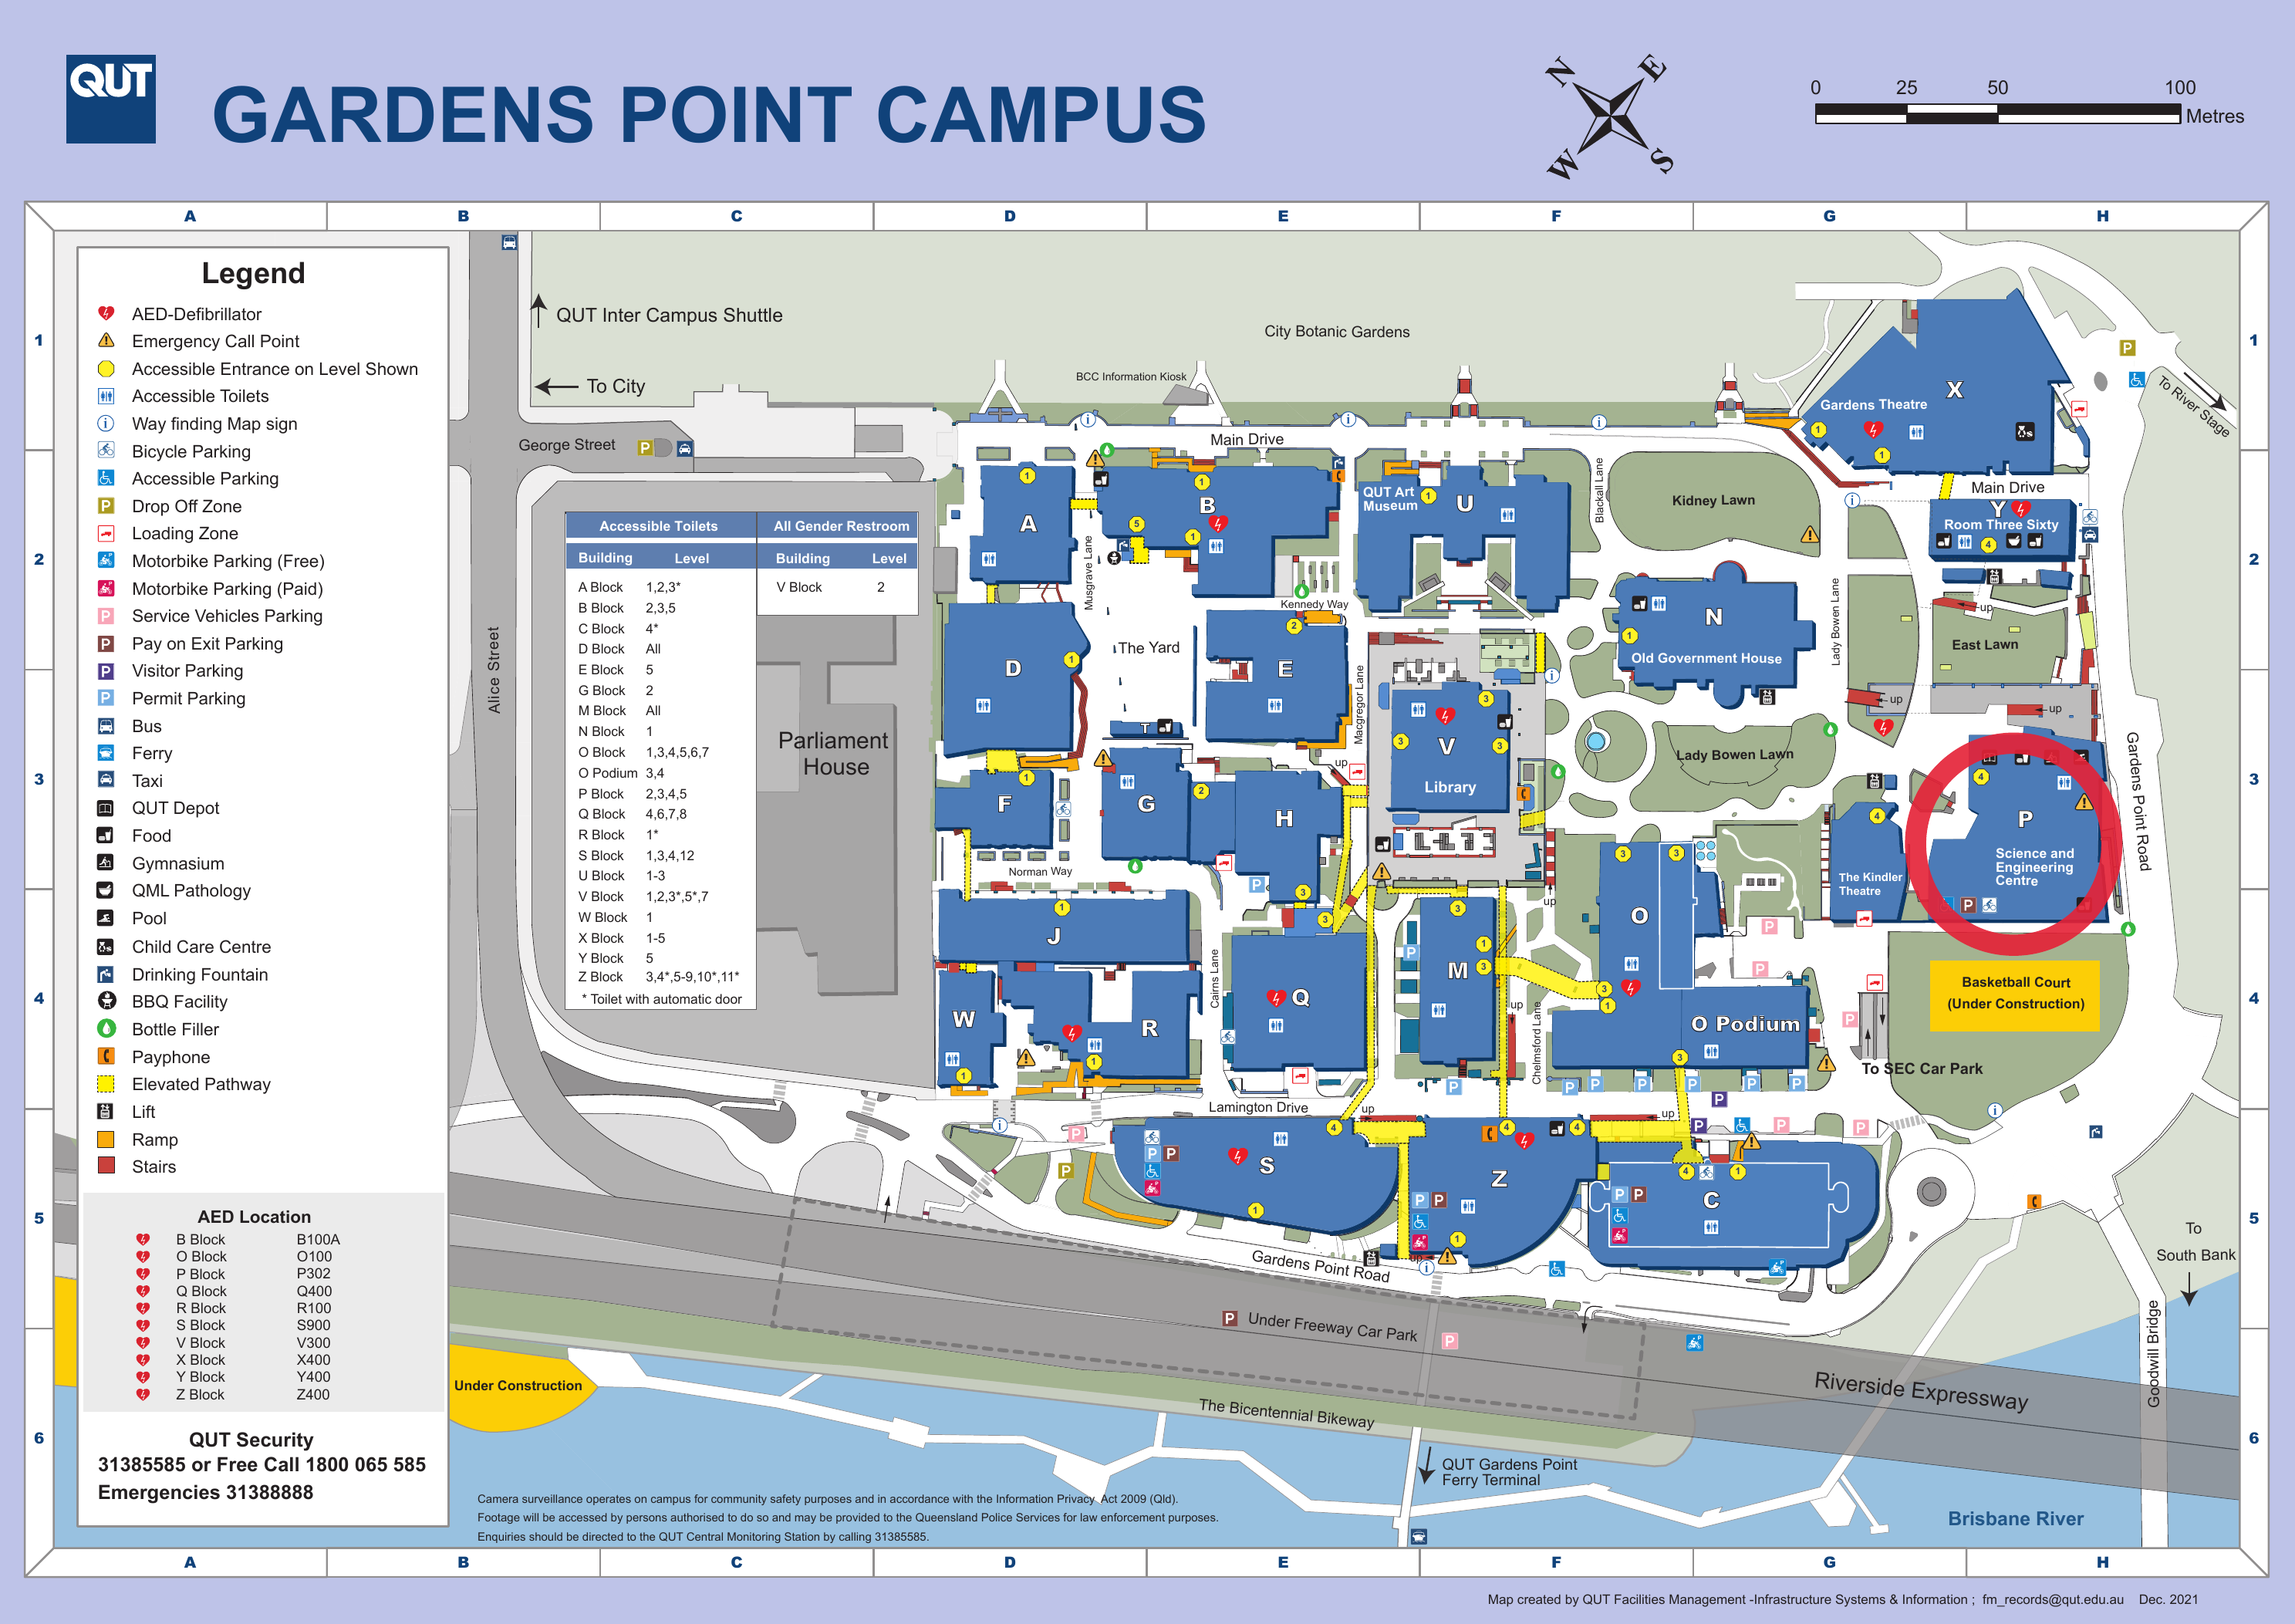
\includegraphics[width=0.8\textwidth,keepaspectratio]{pics/rendered-pdf/QUT-Brisbane-Maps-1.png}
	\caption{QUT G.P. 校区的地图}
\end{figure}

\subsubsection{关于你们的先驱者}\footnotemark
\footnotetext{这里的“先驱者”泛指已经赴澳学习的学长学姐。由于目前没有学姐的照片，暂以现有资料为主，敬请见谅。}
G23 缪彭哲学长和 G23 尤嘉晨学长已经先行赴澳，在 QUT 开启了与袋鼠“自由搏击”的留学生活。

\begin{figure}[H]
	\centering
	
	\begin{minipage}[t]{0.34\textwidth}
		\centering
		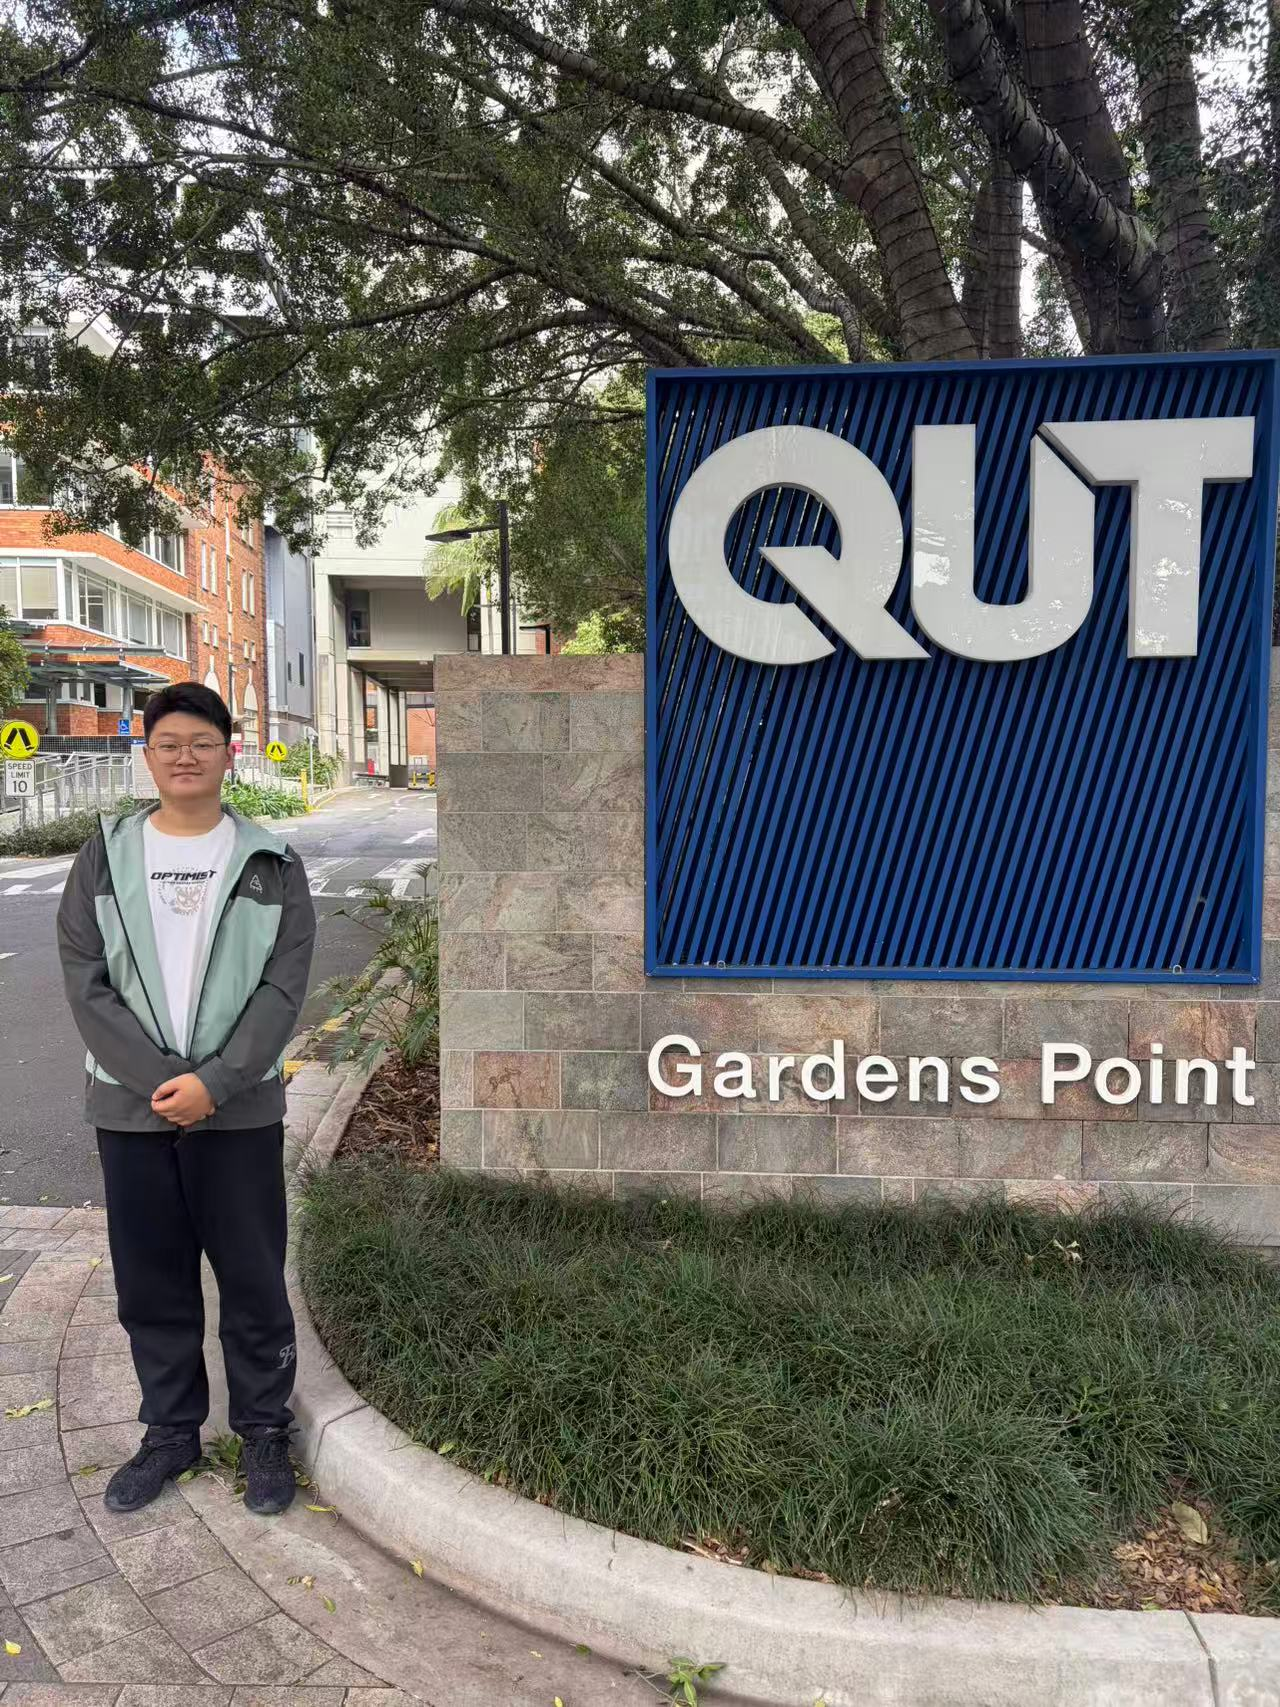
\includegraphics[width=1\linewidth,keepaspectratio]{pics/photo1.jpg}
		\caption{G23缪彭哲学长在 QUT 合影}
	\end{minipage}
	\hfill
	\begin{minipage}[t]{0.6\textwidth}
		\centering
		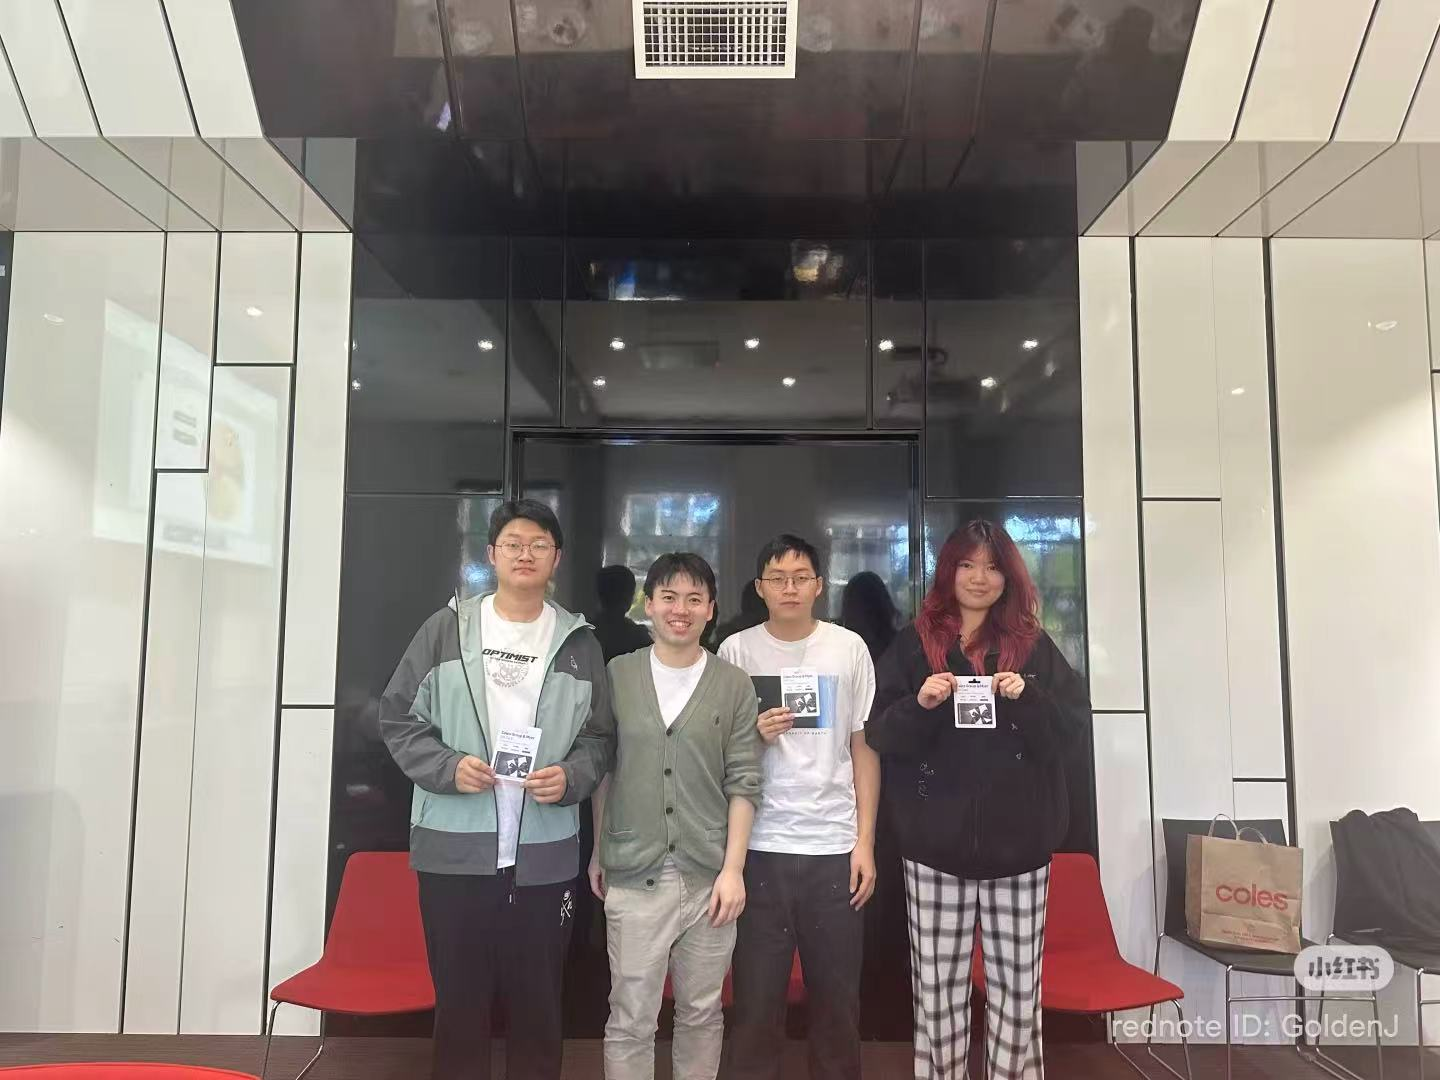
\includegraphics[width=1\linewidth,keepaspectratio]{pics/photo3.jpg}
		\caption{摄于 QUT 中国新生联谊会, G23 缪彭哲 (左 1) 与 G23 尤嘉晨 (左 3)}
	\end{minipage}
	
\end{figure}

\newpage
\subsection{中外合办课程}

下表为学业记录中列出的已获课程豁免的中外合办课程目录. 

\scriptsize
\renewcommand{\arraystretch}{1.15}
\begin{longtable}{p{0.22\textwidth}p{0.62\textwidth}p{0.06\textwidth}}
\toprule
QUT Unit 代码 & 课程名称 & 学分 \\
\midrule
\endhead
\bottomrule
\endfoot
\rowcolor{white}
\multicolumn{3}{l}{\textbf{大一下学期}}\\
\rowcolor{white}
\texttt{IFB102} & Introduction to Computer Systems & 12 \\
\rowcolor{white}
\texttt{IFB105} & Database Management & 12 \\
\rowcolor{gray!15}
\multicolumn{3}{l}{\textbf{大二上学期}}\\
\rowcolor{gray!15}
\texttt{IFB103} & IT Systems Design & 12 \\
\rowcolor{gray!15}
\texttt{IFB104} & Introduction to Programming (Building IT Systems) \footnotemark & 12 \\
\rowcolor{white}
\multicolumn{3}{l}{\textbf{大二下学期}}\\
\rowcolor{white}
\texttt{IAB207} & Rapid Web Application Development & 12 \\
\rowcolor{white}
\texttt{IFB201} & Introduction to Enterprise Computing & 12 \\
\rowcolor{white}
\texttt{CAB201} & Object-Oriented Programming and Design (Programming Principles) & 12 \\
\rowcolor{gray!15}
\multicolumn{3}{l}{\textbf{大三上学期}}\\
\rowcolor{gray!15}
\texttt{IAB203} & Process Modelling (Business Process Modelling) & 12 \\
\rowcolor{gray!15}
\texttt{IAB230} & Design of Enterprise IoT & 12 \\
\rowcolor{gray!15}
\texttt{IAB201} & Modelling Techniques for Information Systems & 12 \\
\rowcolor{gray!15}
\texttt{CAB222} & Networks & 12 \\
\rowcolor{white}
\multicolumn{3}{l}{\textbf{大三下学期}}\\
\rowcolor{white}
\texttt{IFB240} & Cyber Security & 12 \\
\rowcolor{white}
\texttt{IAB305} & IT Strategy and Management (Information Systems Lifecycle Management) & 12 \\
\rowcolor{white}
\texttt{IAB204} & Business Analysis for IT Systems (Business Requirements Analysis) & 12 \\
\end{longtable}
\normalsize

这些课将会在JIT进行教学, 教学方式为中方老师行日常教学, 每个课程的外方教师需要在每学期末来访JIT, 进行为期1周的教学, 教学通常为英文教学. 所以最后放寒暑假普遍比较晚.

\footnotetext{注: 括号内为旧名称. 为了同一课程名称, 后文中课程信息均使用旧名称.}



\newpage
\subsection{快速了解一下 JIT}

\official{https://www.jit.edu.cn/xxgk/xxjj.htm}{金陵科技学院 (JIT, Jinling Institute of Technology)} 坐落于六朝古都南京, 是一所以培养高素质应用型人才为主要任务的公办全日制普通本科院校, 是教育部应用科技大学改革试点战略研究单位, 中国应用技术大学 (学院) 联盟创始单位, 长三角地区应用型本科高校联盟主席单位, 江苏省一流应用型本科高校建设单位.

金陵科技学院江宁校区的最新图, 已给各位搓好, 请查看附录~\ref{app:jit-map}. 


\subsubsection{JIT 学校生活常用网站}

\begin{itemize}[itemsep=0.1em,topsep=0.25em,parsep=0pt,partopsep=0pt]
 \item \official{https://www.jit.edu.cn/}{金陵科技学院官网}: 查看学校新闻, 通知和相关部门入口.
 \item \official{https://jwxt.jit.edu.cn/default2.aspx}{学校教务系统}: 查询个人课表, 成绩及选课信息, 按教务通知完成选课等操作.
\end{itemize}

\subsubsection{快速了解一些事项}

\paragraph{校园跑} 目前大一, 大二的校园跑会计入当学期的体育成绩. 根据个人记忆, 大一是强制性打卡 (不跑体育课会挂科), 大二没有强制要求, 但这是体育成绩与综测成绩的一部分. 详细参考附录~\ref{app:school-running}.
\paragraph{四六级} 根据国教院的要求, 四级是毕业的刚性要求. 请在大一还没变成澄澈大学生之前赶快考. 很好过, 根据个人记忆, 裸考可过 (取决于人), 而六级并不是刚性要求.
\paragraph{计算机等级考试} 作为计算机相关专业的学生, 我们不需要考计算机等级考试.
\paragraph{出国问题} 毋庸置疑, 项目强制要求出国.
\paragraph{选课问题} 国教院公选课的毕业要求不低于 6.5 学分, 同时每个学生在校期间必须选修一门美育课程.
\paragraph{外方课} 外方课是指由 QUT 开发的课程, 一般先由中方老师上 8 周的课程, 这 8 周我们称为中方课, 之后 (一般是之后) 由 QUT 指派老师飞往 JIT 上连续一周的课 (从早到晚), 并在最后一天进行考试 (如果有), 但是最终成绩由中方老师评定, 所以即便中方老师讲的内容与外方老师讲的内容不同, 也要好好上课.
\paragraph{雅思要求} 雅思成绩的有效期为 2 年, 所以建议各位在大二升大三的暑假考一下. 现在也可以先考一次试试水. 要求是总分不低于 6.5, 单项不低于 6.0. 请参考\official{https://www.qut.edu.au/courses/bachelor-of-information-technology-business-analysis-and-it-management\#requirements}{QUT 语言要求部分}. 未达标可以参考附录~\ref{app:ielts-requirement} 参加语言班.
\paragraph{学费生活费} QUT 阶段的学费, 日常开销, 住宿价格和学期时间安排见第~\ref{sec:qut-life}~节以及附录~\ref{app:qut-fees}--\ref{app:qut-calendar}.
\paragraph{加入校学生会} 关注微信公众号``金科青年'' 这个是校学生会的公众号. 上面会有招募信息. 同时南北食堂展板上会有二维码. 扫码报名. 也可以直接查看\official{https://v.wjx.cn/vm/er5UZFS.aspx}{校学生会招新报名表}, 并加入\official{https://qun.qq.com/universal-share/share?ac=1\&authKey=I5eYrINXEBmTFLU95VOyw7WRxbTO1EXW0e0E9Ge0ngoXddnkwDEWhcUuHadg/x6/\&busi\%5Fdata=eyJncm91cENvZGUiOiIxMTIxMDQ4NjI5IiwidG9rZW4iOiJuVkZ3YzZ0NWFnNDNWMmU2NC9kRERoTTJHYitTVDcwSVdFck9vU1YzZ0hZQ3Y1ZUM5ZUJhMzg5aUU1ejRpc1FIIiwidWluIjoiNDgxNzk2MTQzIn0=\&data=ger-r0XXoTIzhEfXo-KOAkTCkCrl6b1Kf7zOUPAkPKdlHGlOowzXERxr9dG-wpPiYuV14nhLLbcrWMEOONF18Wc66SlhTDxQrSeM-BiGA8c\&svctype=5\&tempid=h5\%5Fgroup\%5Finfo}{校学生会招新 QQ 群}. 主包以前大一学生会传媒社的, 负责活动摄影. 也欢迎大家踊跃参加!

\paragraph{加入社团} 社团招新会在军训后, 有一个``百团大战''的活动, 是专门来招新的. 其余的招新信息请默认为假消息.

\paragraph{奖学金} G26 JIT 奖学金是根据综测排名以及成绩具体考虑, 请具体参考软件程学院相关政策. QUT 奖学金展现于学费的减免. 有两种, 分别为25\%减免和20\%减免. 详细可以参考 \official{https://www.qutchina.cn/scholarship}{QUT 奖学金}. 据缪学长反馈, 第四年在QUT大部分都获取两种奖学金的其中一种. 


\newpage

\section{每学期课程}
\subsection{大一上学期}
请注重数学科目的考试以及 C 语言编程. 最好在军训期间学会 C 语言的编程基础 (基本算法逻辑), 后续再研究指针以及寄存器相关的知识. 建议在上半学期学习 Python (区别于严格数据类型的语言, 方便后续比赛和科研, 大二上学期会开设相关课程) 以及 C++ (一般情况下, 考试如果允许使用 C, 通常也会提供 C++ 编译器, 用该语言可以调用 STL 库, 会更方便). 

\course{高等数学 A1}{4.5}
考核方式: 考试. 主要学习积分等内容. 推荐猴博士的网课作预习, 其他时间上课认真听, 过一遍课本. 有一本``普林斯顿微积分原本''可以看看, 比较容易懂. \official{https://pan.baidu.com/s/19nuSMPd-VwQmOLA8FP-UjQ?pwd=limo}{百度网盘}
\course{线性代数与空间解析几何}{3}
考核方式: 考试. 主要是注意矩阵计算时不要出错. 推荐猴博士的网课作预习, 其他时间上课认真听, 过一遍课本. \official{https://pan.baidu.com/s/147pCVg0qU6LHLsiX5SJvoQ?pwd=limo}{百度网盘}
\course{高级语言编程}{2.5}
考核方式: 上机 C 语言编程, 期末考试. 推荐 \official{https://www.runoob.com/cprogramming/c-tutorial.html}{菜鸟教程} 过一遍里面所有知识. 
\course{高级语言编程实验}{2}
考核方式: 上机 C 语言编程, 黄金考. 建议刷一遍 \official{https://pintia.cn/}{PTA} 里面对应书里面的题目, 以及开放的题目都可以刷. 练出手感, 尝试使用 C++.
\course{IELTS I}{3}
考核方式: 阅读考试, 英文演讲. 没啥, 上课认真听, 别睡觉.
\course{IELTS Speaking I}{1.5}
考核方式: 口语考试 (仿真 P1 和 P2). 没啥, 上课认真听, 别睡觉, 多交流. 
\course{思想道德与法治}{3}
考核方式: 学习通考试. 没啥, 上课认真听.
\course{形势与政策 1}{0.25}
考核方式: 小论文. 没啥, 上课认真听.
\course{心理健康教育}{2}
考核方式: 考查. 没啥, 上课认真听, 别旷课, 别睡觉.
\course{基础课 (体育1)}{1}
考核方式: 体育考试.
\newpage
\subsection{大一下学期}
如果 C++ 和 Python 学得不错, 有兴趣的话可以深入学习一下算法. 可以参考 \official{https://www.hello-algo.com/}{Hello 算法} 入个门, 后面去 \official{https://www.acwing.com/}{AcWing} 和 \official{https://www.luogu.com.cn/}{洛谷} 上继续深造一下. 
\subsubsection{国内课程}
\course{高等数学 A2}{5.5}
考核方式: 考试. 主要学习积分等内容. 推荐猴博士的网课作预习, 其他时间上课认真听. 重点是过一遍课本, 书本内容已经比较浅显. \official{https://pan.baidu.com/s/19nuSMPd-VwQmOLA8FP-UjQ?pwd=limo}{百度网盘}
\course{概率论与数理统计 A}{3}
考核方式: 考试. 过一遍书. 如果想往人工智能方向学习, 这门课建议认真学一些内容, 多看点课程, 有利于后续学习机器学习. \official{https://pan.baidu.com/s/185jk4duUJqrre\_G-8NcbhA?pwd=limo}{百度网盘}
\course{离散结构}{3}
考核方式: 考试. 过一遍书基本上没事. 可以到 B 站上随便看点课程, 但最好学到点真东西, 对大二的数据结构有帮助, 对大三的操作系统也有帮助. 最好学点吧, 求求了.
\course{IELTS Elementary Listening and Reading}{2}
考核方式: 考试 (听力 + 阅读). 没啥, 上课认真听, 别睡觉.
\course{IELTS Elementary Writing}{2}
考核方式: 考试 (P1 写作). 没啥, 上课认真听, 别睡觉.
\course{IELTS Elementary Speaking}{2}
考核方式: 口语考试 (仿真 P3). 没啥, 上课认真听, 别睡觉, 多交流. 
\course{军事理论概论}{2}
考核方式: 开卷考试. 没啥, 上课认真听. 
\course{中国近现代史纲要}{3}
考核方式: 学习通考试. 没啥, 上课认真听. 
\course{形势与政策 2}{0.25}
考核方式: 小论文. 没啥, 上课认真听. 
\course{大学生劳动教育}{0.5}
考核方式: 考查. 没啥, 上课认真听. 
\course{基础课 (体育2)}{1}
考核方式: 体育考试.



\subsubsection{外方课程}
\course{Introduction to Computer Systems (计算机系统概论)}{3}
考核方式: 中方 (写报告); 外方 (做树莓派项目, 写报告, 汇报). 学习 Linux 的指令.
\course{Database Management (数据库原理)}{3}
考核方式: 中方 (写 SQL 报告); 外方 (考试). 建议提前学习一下 SQL 语言以及 ER 图怎么画. 具体外方课是学习 ORM (Object-Role Modeling) 的数据库建模.


\newpage
\subsection{大二上学期}

\subsubsection{国内课程}
\course{软件工程导论}{3}
考核方式: 设计文档, 汇报.
\course{Data Structures and Algorithms (数据结构与算法)}{4}
考核方式: 上机考试.
\course{大学物理 C}{4}
考核方式: 考试.
\course{大学物理实验 1}{1}
考核方式: 写报告.
\course{IELTS Writing}{2}
考核方式: 考试 (P1 + P2 写作).
\course{IELTS Listening and Reading}{2}
考核方式: 考试 (听力 + 阅读).
\course{English Language and Culture}{2}
考核方式: 写一篇论文, 采用 APA 格式.
\course{马克思主义基本原理}{3}
考核方式: 学习通考试.
\course{形势与政策 3}{0.25}
考核方式: 小论文.
\course{体育3}{1}
考核方式: 体育考试.

\subsubsection{外方课程}
\course{IT Systems Design (IT 系统设计)}{4}
考核方式: 中方 (写报告); 外方 (写报告). 本课程学习信息系统的架构与设计. 学习前端设计, 建议学会墨刀或者Figma来画原型图. 学会画 Fundamental Modeling Concepts (FMC) 图.
\course{Building IT Systems (IT 系统架构)}{3}
考核方式: 中方 (Python 实验报告); 外方 (考试). 本课程已改名为 Introduction to Programming, 主要学习 Python.

\newpage
\subsection{大二下学期}

\subsubsection{国内课程}
\course{数学建模}{3}
考核方式: 考试+实验报告. 实验报告部分为MatLab.
\course{Academic English}{2}
考核方式: 写小论文.
\course{Communicative English}{2}
考核方式: 报告.
\course{毛泽东思想和中国特色社会主义理论体系概论}{3}
考核方式: 学习通考试.
\course{形势与政策 4}{0.25}
考核方式: 小论文.
\course{体育4}{1}
考核方式: 体育考试.

\subsubsection{外方课程}
\course{Rapid Web Application Development (快速网络应用程序开发)}{3}
考核方式: 中方 (考查); 外方 (报告, 加项目展示). 本课程学习使用Flask开发网站.
\course{Introduction to Enterprise Systems (企业系统导论)}{3}
考核方式: 中方 (写报告); 外方 (写报告, 考试).
\course{Programming Principles (编程原理)}{3}
考核方式: 中方 (写报告); 外方 (写代码, 考试). 本课程改名为 Object-Oriented Programming and Design 但内容不变, 学习C\#.

\newpage
\subsection{大三上学期}

\subsubsection{国内课程}
\course{计算机系统基础}{2}
考核方式: 小测+考试+实验报告+调研报告. 本课程相对较难, 容易挂科, 一定要好好学, 同时没有平时分, 全看你的成绩.
\course{操作系统}{3}
考核方式: 考试+实验报告. 本课程相对较难 (没有上面那个难), 实验部分为Linux.
\course{软件质量保证与测试}{3}
考核方式: 考试+实验报告. 没啥, 上课认真听. 
\course{软件测试技术课程设计}{1}
考核方式: 实验报告+汇报. 本课程要结合上面一门课所学的知识, 对自己开发的一款软件进行全面的测试.
\course{计算机网络课程设计}{1.5}
考核方式: 实验报告+考试. 本课程使用Packet Tracer对网络的基本架构以及路由器交换机的部署进行了解, 可以为下学期的网络做基础, 期末考试会每人随机抽取一道网络部署题, 在有限的时间内完成, 考试后, 根据你的题目完成一份实验部署报告.
\course{习近平新时代中国特色社会主义思想概论}{3}
考核方式: 学习通考试.

\subsubsection{外方课程}
\course{Business Process Modelling (商业过程建模)}{3}
考核方式: 报告+考试. 本课程已改名为Process Modelling, 主要学习 BPMN, 并利用这门建模语言对一些流程进行建模. 报告内容需要完成的比较多, 考试相对简单.
\course{Design of Enterprise IoT (企业物联网设计)}{3}
考核方式: 报告+汇报. 本课程学习一些物联网的基本内容, 每组需要选择一个企业问题, 为此设计一套物联网系统. 本课程可能先上外方课, 到期末才安排中方课, 会在期末提前开启下学期的专业方向课程设计的前半部分. (G23情况)
\course{Modelling Techniques for Information Systems (信息系统建模技术)}{3}
考核方式: 报告+考试. 本课程学习两种建模语言 (ERD与Petri Net), 你要用这两种语言完成两个报告, 考试相对简单.
\course{Networks (网络)}{3}
考核方式: 报告+实验考试+理论考试. 本课程学习网络的相关知识, 实验考试考子网划分与网络纠错, 理论考试考课程学的一些基础理论, 都为纸笔考试. 报告你将使用Wireshark对一段异常流量进行分析, 并提出解决方案.

\newpage
\subsection{大三下学期 (G23 参考)}

\subsubsection{国内课程}
\course{专业方向课程设计}{3}
考核方式: 报告+汇报. 本课程会给你一个主题, 以小组为单位从零完成一个项目 (从可行性分析到测试), 可能会在上一个学期完成设计部分, 并在本学期完成编码部分.
\course{软件设计与体系结构}{3}
考核方式: 实验+考试. 没啥, 上课认真听. 
\course{Management (管理学)}{3}
考核方式: 报告+考试. 本课程你将学习管理学的四个基本职能, 课程为中英双语教学, 报告和考试均为英文, 每周会给一个主题, 完成一份一页的报告, 每完成一章节, 会发布书本配套题库, 一定要好好看, 考试100\%是原题. 此课程为商学院开设, 并非外方课.

\subsubsection{外方课程}
\course{Cybersecurity (网络安全)}{3}
考核方式: 考试. 本课程你将学习到网络安全的基本理论, 偏介绍性质.
\course{Information Systems Lifecycle Management (信息系统生命周期管理)}{3}
考核方式: 报告+考试. 本课程已改名为IT Strategy and Management, 课程探讨利用商业模式和商业案例分析, 从宏观层面提出并论证信息系统方案. 课程考试比较偏理论, 需要对上课的理论进行记忆.
\course{Business Requirements Analysis (企业数据挖掘)}{3}
考核方式: 报告+考试. 本课程已改名为Business Analysis for IT Systems, 将介绍业务分析师所需的角色, 知识, 技能与方法, 重点讲解业务分析师使用的工具与方法, 以及创造力和沟通能力等软技能.

\newpage
\subsection{第四年QUT课程}

本项目采用``3+1''课程路径: 前三年在金陵科技学院完成国内阶段学习, 最后一年赴 QUT 学习信息技术学士阶段课程. QUT 最后一年可以从信息技术专业方向中选择一个 Major, 并按该方向完成专业课程. 以及完成Minor辅修专业的课程和公共课.

\subsubsection{IT Major}

\paragraph{QUT 最后一年可选择的专业方向}
QUT 信息技术专业的 Major Options 包括以下方向 (括号内为英文名称, 其中前四个方向无法选择\footnotemark): 

\begin{itemize}[itemsep=0.1em,topsep=0.25em,parsep=0pt,partopsep=0pt]
	\item \unavailablemajor{人工智能 (Artificial Intelligence Major); }
	\item \unavailablemajor{计算机科学 (Computer Science Major); }
	\item \unavailablemajor{网络安全 (Cyber Security Major); }
	\item \unavailablemajor{软件开发 (Software Development Major); }
	\item 商业分析与 IT 管理 (Business Analysis and IT Management Major); 
	\item 企业计算 (Enterprise Computing Major); 
	\item 流程分析与自动化 (Process Analytics and Automation Major); 
\end{itemize}
\footnotetext{“无法选择”仅指本项目当前的 JIT--QUT 衔接安排，不代表 QUT 的普遍限制；最终 Major, 补修要求和课程负荷以个人 Advanced Standing, 开课安排及 QUT 批准的 Study Plan 为准。详见 \official{https://www.qut.edu.au/courses/bachelor-of-information-technology-enterprise-computing}{QUT BIT 页面}和\official{https://www.qut.edu.au/study/international/study-abroad-program/what-can-i-study}{官方说明}。}

\paragraph{三项专业方向及课程 (\checkmark 表示已在国内修过的课程)}
\mbox{}\par
\textbf{企业计算}~\texttt{IN01MJR-ENTCOM}\par
\textit{Enterprise Computing Major}\par
\scriptsize
\renewcommand{\arraystretch}{1.15}
\begin{longtable}{p{0.22\textwidth}p{0.62\textwidth}p{0.06\textwidth}}
	\toprule
	QUT Unit 代码 & 课程名称 & 学分 \\
	\midrule
	\endhead
	\bottomrule
	\endfoot
	\texttt{IAB401} & \official{https://www.qut.edu.au/study/unit?unitCode=IAB401}{Enterprise Architecture} & 12 \\
	\texttt{IAB207} & \completedcourse{https://www.qut.edu.au/study/unit?unitCode=IAB207}{Rapid Web Application Development} & 12 \\
	\texttt{CAB201} & \completedcourse{https://www.qut.edu.au/study/unit?unitCode=CAB201}{Object-Oriented Programming and Design} & 12 \\
	\texttt{IAB251} & \official{https://www.qut.edu.au/study/unit?unitCode=IAB251}{Software Engineering for Enterprise Systems} & 12 \\
	\texttt{IAB330} & \official{https://www.qut.edu.au/study/unit?unitCode=IAB330}{Applied Internet of Things} & 12 \\
	\texttt{--} & \official{https://www.qut.edu.au/courses/bachelor-of-information-technology-enterprise-computing}{当届选项清单 (任选 1 门)}; 具体 Unit code 以 Study Plan 显示为准 & 12 \\
\end{longtable}
\normalsize

\textbf{商业分析与 IT 管理}~\texttt{IN01MJR-BAITMG}\par
\textit{Business Analysis and IT Management Major}\par
\scriptsize
\renewcommand{\arraystretch}{1.15}
\begin{longtable}{p{0.22\textwidth}p{0.62\textwidth}p{0.06\textwidth}}
	\toprule
	QUT Unit 代码 & 课程名称 & 学分 \\
	\midrule
	\endhead
	\bottomrule
	\endfoot
	\texttt{IAB203} & \completedcourse{https://www.qut.edu.au/study/unit?unitCode=IAB203}{Process Modelling} & 12 \\
	\texttt{IAB204} & \completedcourse{https://www.qut.edu.au/study/unit?unitCode=IAB204}{Business Analysis for IT Systems} & 12 \\
	\texttt{IAB305} & \completedcourse{https://www.qut.edu.au/study/unit?unitCode=IAB305}{IT Strategy and Management} & 12 \\
	\texttt{IAB353} & \official{https://www.qut.edu.au/study/unit?unitCode=IAB353}{Data Analytics for Enterprise Systems} & 12 \\
	\texttt{IAB401} & \official{https://www.qut.edu.au/study/unit?unitCode=IAB401}{Enterprise Architecture} & 12 \\
	\texttt{IAB402} & \official{https://www.qut.edu.au/study/unit?unitCode=IAB402}{IT Consulting and Leadership} & 12 \\
\end{longtable}
\normalsize

\newpage
\textbf{流程分析与自动化}~\texttt{IN01MJR-PANAUT}\par
\textit{Process Analytics and Automation Major}\par
\scriptsize
\renewcommand{\arraystretch}{1.15}
\begin{longtable}{p{0.22\textwidth}p{0.62\textwidth}p{0.06\textwidth}}
	\toprule
	QUT Unit 代码 & 课程名称 & 学分 \\
	\midrule
	\endhead
	\bottomrule
	\endfoot
	\texttt{IAB203} & \completedcourse{https://www.qut.edu.au/study/unit?unitCode=IAB203}{Process Modelling} & 12 \\
	\texttt{IAB201} & \completedcourse{https://www.qut.edu.au/study/unit?unitCode=IAB201}{Modelling Techniques for Information Systems} & 12 \\
	\texttt{DSB202} & \official{https://www.qut.edu.au/study/unit?unitCode=DSB202}{Data Ethics and Society} & 12 \\
	\texttt{IAB320} & \official{https://www.qut.edu.au/study/unit?unitCode=IAB320}{Process Improvement} & 12 \\
	\texttt{IAB321} & \official{https://www.qut.edu.au/study/unit?unitCode=IAB321}{Process Technologies} & 12 \\
	\texttt{DSB201} & \official{https://www.qut.edu.au/study/unit?unitCode=DSB201}{Advanced Databases} & 12 \\
	\texttt{IAB204} & \completedcourse{https://www.qut.edu.au/study/unit?unitCode=IAB204}{Business Analysis for IT Systems} & 12 \\
	\texttt{IAB353} & \official{https://www.qut.edu.au/study/unit?unitCode=IAB353}{Data Analytics for Enterprise Systems} & 12 \\
\end{longtable}
\normalsize

\subsubsection{IT 公共课程}

\scriptsize
\renewcommand{\arraystretch}{1.15}
\begin{longtable}{p{0.22\textwidth}p{0.62\textwidth}p{0.06\textwidth}}
	\toprule
	QUT Unit 代码 & 课程名称 & 学分 \\
	\midrule
	\endhead
	\bottomrule
	\endfoot
	\texttt{IFB102} & \completedcourse{https://www.qut.edu.au/study/unit?unitCode=IFB102}{Introduction to Computer Systems} & 12 \\
	\texttt{IFB103} & \completedcourse{https://www.qut.edu.au/study/unit?unitCode=IFB103}{IT Systems Design} & 12 \\
	\texttt{IFB104} & \completedcourse{https://www.qut.edu.au/study/unit?unitCode=IFB104}{Introduction to Programming} & 12 \\
	\texttt{IFB105} & \completedcourse{https://www.qut.edu.au/study/unit?unitCode=IFB105}{Database Management} & 12 \\
	\texttt{IFB201} & \completedcourse{https://www.qut.edu.au/study/unit?unitCode=IFB201}{Introduction to Enterprise Computing} & 12 \\
	\texttt{IFB220} & \official{https://www.qut.edu.au/study/unit?unitCode=IFB220}{Introduction to AI for IT Professionals} & 12 \\
	\texttt{IFB240} & \completedcourse{https://www.qut.edu.au/study/unit?unitCode=IFB240}{Cyber Security} & 12 \\
	\texttt{IFB398} & \official{https://www.qut.edu.au/study/unit?unitCode=IFB398}{IT Capstone Project (Phase 1)\footnotemark} \footnotetext{该课程是在第四年第一学期必修的科目.}& 12 \\
	\texttt{IFB399} & \official{https://www.qut.edu.au/study/unit?unitCode=IFB399}{IT Capstone Project (Phase 2)\footnotemark} \footnotetext{该课程是在第四年第二学期必修的科目.} & 12 \\
\end{longtable}
\normalsize

\subsubsection[IT Minor]{IT Minor\footnotemark}

当前提供以下 11 个 IT Minor 选项. 每个 Minor 为 48 cp, 通常由 4 门, 每门 12 cp 的 Unit 构成.

\scriptsize
\renewcommand{\arraystretch}{1.15}
\begin{longtable}{p{0.20\textwidth}p{0.64\textwidth}p{0.06\textwidth}}
	\toprule
	系统代码 & Minor 名称 & 学分 \\
	\midrule
	\endhead
	\bottomrule
	\endfoot
	\texttt{IN01MNR-ARTINT} & \official{https://www.qut.edu.au/study/options/university-wide-second-majors-and-minors\#minor-multimedia-and-information-technology}{人工智能 (Artificial Intelligence Minor)} & 48 \\
	\texttt{IN01MNR-BAITMG} & \official{https://www.qut.edu.au/study/options/university-wide-second-majors-and-minors\#minor-multimedia-and-information-technology}{商业分析与 IT 管理 (Business Analysis and IT Management Minor)} & 48 \\
	\texttt{IN01MNR-COMASI} & \official{https://www.qut.edu.au/study/options/university-wide-second-majors-and-minors\#minor-mathematical-sciences}{计算数学与仿真 (Computational Mathematics and Simulation Minor)} & 48 \\
	\texttt{IN01MNR-COMPSC} & \official{https://www.qut.edu.au/study/options/university-wide-second-majors-and-minors\#minor-multimedia-and-information-technology}{计算机科学 (Computer Science Minor)} & 48 \\
	\texttt{IN01MNR-CYBSEC} & \official{https://www.qut.edu.au/study/options/university-wide-second-majors-and-minors\#minor-multimedia-and-information-technology}{网络安全 (Cyber Security Minor)} & 48 \\
	\texttt{IN01MNR-DATSCI} & \official{https://www.qut.edu.au/study/options/university-wide-second-majors-and-minors\#minor-data-science}{数据科学 (Data Science Minor)} & 48 \\
	\texttt{IN01MNR-ENTCOM} & \official{https://www.qut.edu.au/study/options/university-wide-second-majors-and-minors\#minor-multimedia-and-information-technology}{企业计算 (Enterprise Computing Minor)} & 48 \\
	\texttt{IN01MNR-HUMCOM} & \official{https://www.qut.edu.au/study/options/university-wide-second-majors-and-minors\#minor-multimedia-and-information-technology}{以人为本的计算 (Human-Centred Computing Minor)} & 48 \\
	\texttt{IN01MNR-INTHGS} & \official{https://www.qut.edu.au/study/options/university-wide-second-majors-and-minors\#minor-multimedia-and-information-technology}{物联网 (Internet of Things Minor)} & 48 \\
	\texttt{IN01MNR-PANAUT} & \official{https://www.qut.edu.au/study/options/university-wide-second-majors-and-minors\#minor-multimedia-and-information-technology}{流程分析与自动化 (Process Analytics and Automation Minor)} & 48 \\
	\texttt{IN01MNR-SOFDEV} & \official{https://www.qut.edu.au/study/options/university-wide-second-majors-and-minors\#minor-multimedia-and-information-technology}{软件开发 (Software Development Minor)} & 48 \\
\end{longtable}

\footnotetext{注意: Minor 方向不能和选择的专业方向相同.}
\normalsize


\section{QUT生活}\label{sec:qut-life}

本节主要介绍赴 QUT 学习期间的学期节奏, 日常开销和住宿选择. 具体安排以 QUT 当年的 Academic Calendar, 个人 Study Plan 和实际租房合同为准.

\subsection{2027年学期节奏}

QUT 2027 年 Semester 1 从 2 月 22 日持续到 6 月 19 日, Semester 2 从 7 月 19 日持续到 11 月 13 日. 这些日期可以用来估算在布里斯班的住宿和生活天数; 完整日历见附录~\ref{app:qut-calendar}.

\paragraph{人民币换算口径} 本节人民币金额统一按 2026 年截至本指南更新时平均汇率 1 澳元约等于人民币 4.80 元粗略换算. 该汇率参考 \official{https://www.exchange-rates.org/exchange-rate-history/aud-cny-2026}{2026 年 AUD/CNY 历史汇率汇总}; 只用于比较预算, 不代表付款时的实时汇率, 也未计入银行卡, 换汇平台或信用卡手续费.

\scriptsize
\renewcommand{\arraystretch}{1.15}
\begin{longtable}{p{0.25\textwidth}p{0.28\textwidth}p{0.37\textwidth}}
\toprule
项目 & 日期 & 备注 \\
\midrule
\endhead
\bottomrule
\endfoot
Semester 1 & 2027-02-22--2027-06-19 & Final grades 于 2027-07-02 发布 \\
Semester 1 补考/延期考试 & 2027-07-17--2027-07-31 & 具体是否需要参加取决于个人成绩 \\
Semester 2 & 2027-07-19--2027-11-13 & Final grades 于 2027-11-26 发布 \\
Semester 2 补考/延期考试 & 2028-01-10--2028-01-22 & 需要时再按学校通知参加 \\
\end{longtable}
\normalsize

\subsection{日常生活费}

据缪彭哲学长的经验, 日常开销约为每天 A\$30--40 (约人民币 144--192 元), 其中包括伙食. 如果按一个约 17 周的正式学期, 约 119 天计算, 不含房租和学费, 一个学期约需 A\$3,570--4,760 (约人民币 17,136--22,848 元); 两个正式学期合计约为 A\$7,140--9,520 (约人民币 34,272--45,696 元). 这只是生活费的经验预算, 手机, 交通, 教材, 娱乐和旅行等额外支出需要另行预留.

住宿方面, 学长提供的经验价格为: 稍微好一些的 ensuite 房间约 A\$450/周 (约人民币 2,160 元/周), twin 类型房间约 A\$200/周 (约人民币 960 元/周). 如果按 52 周租期, 分别约为 A\$23,400/年 (约人民币 11.23 万元) 和 A\$10,400/年 (约人民币 4.99 万元). 签约前应确认租期, 押金, 账单, 家具, 网络和退租条款.

\subsection{机票预算}

机票价格受出发城市, 购票时间, 是否直飞, 行李和寒暑假影响很大. 以当前查询结果作为参考, 上海 (PVG)--布里斯班 (BNE) 经济舱直飞, 开学及假期等出行高峰期单程票价约为人民币 5,000 元, 淡季约为人民币 3,000 元. 实际价格会随出行日期和购票时间变化. (价格参考去哪儿旅行)

\subsection{QUT附近住宿价格}

QUT Gardens Point 校区附近主要看 Brisbane City 一带, QUT Kelvin Grove 校区附近则可看 Kelvin Grove, Herston 等区域. 下面把 QUT 官方住宿信息, Realestate.com.au, Domain, Flatmates, QUT Accommodation Service 和其他学生住宿平台放在一起比较. 样本均为 2026 年 9 月检索时的价格; 房源会随时下架或调价, 以下内容不构成对任何平台或房源的推荐.

\scriptsize
\renewcommand{\arraystretch}{1.15}
\begin{longtable}{p{0.14\textwidth}p{0.22\textwidth}p{0.15\textwidth}p{0.14\textwidth}p{0.18\textwidth}}
\toprule
平台 & 位置/样本 & 标价 & 与 QUT 的关系 & 备注/来源 \\
\midrule
\endhead
\bottomrule
\endfoot
QUT Accommodation Service & 学生住宿/合租指导 & A\$150--500/周 & 靠近校园或公共交通 & 官方给出的不同住宿类型区间; \official{https://www.qut.edu.au/study/student-life/living-in-brisbane/accommodation-in-brisbane}{QUT 住宿说明} \\
REA & 108 Margaret St, Brisbane City, studio & A\$440/周 (约 ￥2,112) & 一街区至 Gardens Point & 家具房; 独立卫浴; \official{https://www.realestate.com.au/property-apartment-qld-brisbane+city-444778660}{房源} \\
REA & 145 Kelvin Grove Road, studio & A\$340/周 (约 ￥1,632) & 靠近 QUT Kelvin Grove & 共用卫生间; 房源说明称含水电和网络; \official{https://www.realestate.com.au/property-studio-qld-kelvin+grove-440531280}{房源} \\
Domain & Kelvin Grove 1-bed/2-bed 中位数 & A\$585/720/周 & QUT Kelvin Grove 周边 & 为区域中位数, 不是单一房源; \official{https://www.domain.com.au/rent/?suburb=kelvin-grove-qld-4059}{区域搜索} \\
Flatmates & Brisbane City, Kangaroo Point 等合租房 & A\$260--690/周 & 有步行至 Gardens Point 的样本 & 部分房源含账单; 房型和设施差异较大; \official{https://flatmates.com.au/rooms/qut-gardens-point?page=1}{区域搜索} \\
QUT StudyStays & Iglu Brisbane, Iglu Kelvin Grove, UniLodge & A\$199--449/周 & 标注 near campus & 学生住宿平台样本; 以页面当前空房和合同为准; \official{https://qut.studystays.com.au/Listings/Search?IsProbe=False\&Page=2\&Rent=2026\&ShouldLogProbeBan=True}{平台搜索} \\
UQ Rentals & 23--25 Tait St, Kelvin Grove, shared room & A\$280--290/周 & 靠近 QUT Kelvin Grove & 学生房源平台样本; 共用卫生间; \official{https://rental.uq.edu.au/Advert/4132}{房源} \\
\end{longtable}
\normalsize

从这些平台可以看出, 学长所说的 A\$450/周 ensuite 与 Gardens Point 周边的小户型房源处于相近量级; twin 房型的 A\$200/周通常对应合住或共享设施, 不能直接与独立 studio 的价格比较. 预算时建议同时查看至少两个平台, 并把房租, 水电网, 交通和一次性搬入费用分开计算.

PS: 学生公寓一般是包水电网的, 无需担心用量. 而社会公寓一般需要你自己去开通水电网账户, 按量计费.

\subsubsection{学生公寓常见房型}

澳大利亚学生公寓的房型和国内大学宿舍差别比较大. 在查看 UniLodge, Iglu, Scape 等学生公寓时, 经常会看到 Studio, Ensuite, Non-ensuite 和 Twin Share 等名称. 不同公寓对具体户型的命名可能略有差异, 但基本可以按照下面几类理解. 具体图片房型展示请查看附录~\ref{app:room}. 

\scriptsize
\renewcommand{\arraystretch}{1.18}

\begin{longtable}{@{}p{0.10\textwidth}p{0.17\textwidth}p{0.22\textwidth}p{0.26\textwidth}p{0.15\textwidth}@{}}

\toprule

房型 & 卧室/卫浴 & 厨房和公共区域 & 特点 & 布里斯班参考价格 \\

\midrule

\endhead

\bottomrule

\endfoot

Studio & 独立卧室, 独立卫浴 & 通常有自己的独立厨房, 不需要与其他住户共享 & 私密性最高, 基本可以理解为一个人住的小型公寓; 比较适合喜欢独立空间的同学, 部分房型也允许 Couple 入住 & A\$479--529/周 \\

Ensuite & 独立卧室, 独立卫浴 & 与其他室友共享厨房和客厅 & 比较常见的学生公寓房型. 每个人都有自己的卧室和卫生间, 卧室通常带独立门锁; 一套房一般住约 4--6 人 & A\$389--459/周 \\

Non-ensuite & 独立卧室, 共用卫浴 & 与其他室友共享厨房和客厅 & 拥有自己的卧室, 但卫生间也需要和室友共用. 私密性比 Ensuite 略低, 但通常价格更便宜, 性价比较高; 一套房一般住约 4--6 人 & A\$299--439/周 \\

Twin Share & 两人共享同一卧室 & 通常共用厨房和卫浴; 具体布局视公寓而定 & 一个房间内通常放两张单人床或上下床, 可以理解为类似国内双人宿舍或标间. 适合朋友或同学一起入住, 通常是学生公寓中价格比较低的房型 & A\$239--359/周 \\

\end{longtable}

\normalsize

\subsubsection{澳洲常见床型大小}

澳大利亚学生公寓中的床型名称和国内不完全一样. 租房时经常会看到 Single, King Single, Double, Queen 等名称. 不同公寓实际床垫尺寸可能略有差异, 下面列出澳大利亚常见的参考尺寸.

\scriptsize
\renewcommand{\arraystretch}{1.15}

\begin{longtable}{@{}p{0.14\textwidth}p{0.18\textwidth}p{0.18\textwidth}p{0.40\textwidth}@{}}

\toprule

床型 & 常见尺寸（厘米） & 英制尺寸 & 简单理解 \\

\midrule

\endhead

\bottomrule

\endfoot

Single & 约 92 $\times$ 188 cm & 3'0'' $\times$ 6'2'' & 普通单人床, 学生公寓中比较常见 \\

Single Long & 约 92 $\times$ 203 cm & 3'0'' $\times$ 6'8'' & 宽度和 Single 接近, 但长度更长 \\

King Single & 约 107 $\times$ 203 cm & 3'6'' $\times$ 6'8'' & 比普通 Single 更宽也更长, 学生公寓中非常常见 \\

Double & 约 138 $\times$ 188 cm & 4'6'' $\times$ 6'2'' & 比单人床明显更宽, 一个人睡比较宽松 \\

Queen & 约 153 $\times$ 203 cm & 5'0'' $\times$ 6'8'' & 澳大利亚住宅和公寓中很常见的双人床尺寸 \\

King & 约 183 $\times$ 203 cm & 6'0'' $\times$ 6'8'' & 大型双人床, 学生公寓中相对少见 \\

Super King & 约 203 $\times$ 203 cm & 6'8'' $\times$ 6'8'' & 非常大的双人床, 普通学生公寓中并不常见 \\

\end{longtable}

\normalsize

\subsection{电话卡, 银行卡, 公交卡}
\subsubsection{电话卡}
到澳大利亚后尽快办理一个澳大利亚手机号码. 手机号除了日常通信外, 还经常用于银行验证码, 学校账户, 租房, 外卖和各种网站注册, 因此建议长期保留同一个号码. 

澳大利亚主要移动网络包括 Telstra, Optus 和 Vodafone, 此外还有大量使用这些网络的虚拟运营商. 对于刚到澳大利亚的留学生, 比较常见的选择是 Telstra, Boost Mobile 和 Optus. 

\scriptsize
\renewcommand{\arraystretch}{1.15}
\begin{longtable}{p{0.13\textwidth}p{0.2\textwidth}p{0.15\textwidth}p{0.42\textwidth}}
\toprule
运营商 & 常见套餐 & 网络/特点 & 备注 \\
\midrule
\endhead
\bottomrule
\endfoot
Telstra & A\$44 / 28 天, 20GB & Telstra 网络 & 澳大利亚最大的移动网络运营商之一. 覆盖范围较广, 但价格通常也较高. 适合比较看重网络覆盖和稳定性的同学. \official{https://www.telstra.com.au/mobile-phones/prepaid-mobiles}{Telstra Pre-Paid} \\
Boost Mobile & A\$39 / 28 天, 30GB & Telstra 网络 & 个人比较推荐. 使用 Telstra 网络, 价格通常比 Telstra 本家便宜. A\$39 套餐包括澳大利亚境内标准电话和短信不限量, 并支持未使用流量滚存. Boost 也提供半年和一年有效期的套餐. \official{https://boost.com.au/prepaid-plans}{Boost Prepaid} \\
Optus & 约 A\$39--44 / 28 天 & Optus 网络 & 经常有新用户优惠和额外流量. 套餐价格和活动变化比较频繁, 购买时直接查看官网即可. \official{https://www.optus.com.au/prepaid/sim-plans}{Optus Prepaid} \\
\end{longtable} 
\normalsize

截至 2026 年 9 月, Telstra 的 A\$44 Pre-Paid 套餐包含 20GB 流量; Boost 的 A\$39 套餐正常续费包含 30GB 流量. Boost 还有长期套餐, 例如 A\$300 / 365 天, 240GB, 平均约 A\$25/月, 比较适合确定会在澳大利亚生活一年的同学. 

PS: 运营商经常做新用户促销, 例如首月半价, 额外流量等. 这类活动变化非常快, 本指南不建议按照促销价做长期预算, 实际购买时再看官网. 平时也可以在超市购买打折的电话卡, 同时澳洲电话卡也支持携号转网, 每个月用不同的运营商也是可以的. 

\subsubsection{银行卡}
到澳大利亚后建议至少准备一张澳大利亚本地银行卡. 澳大利亚的日常转账, 工资, 退款, 房租以及部分 Direct Debit 都会使用本地银行账户, 因此中国银行卡不能完全代替澳大利亚银行账户. 

这里主要介绍 Commonwealth Bank (CommBank / CBA) 和中国银行 (澳大利亚). 

简单来说, 可以把常见选择整理成下面这张表. 需要特别注意, \textbf{中国银行 (澳大利亚) 有限公司和中国大陆的中国银行虽然属于同一集团, 但账户并不是同一个账户}; 国内中行卓隽留学信用卡也不是澳大利亚本地 Transaction Account. 

\scriptsize
\renewcommand{\arraystretch}{1.18}
\begin{longtable}{@{}p{0.13\textwidth}p{0.14\textwidth}p{0.29\textwidth}p{0.22\textwidth}p{0.08\textwidth}@{}}
\toprule
产品 & 类型 & 主要用途和功能 & 办理或费用要点 & 建议 \\
\midrule
\endhead
\bottomrule
\endfoot
Commonwealth Bank (CommBank / CBA) &
澳洲本地日常交易账户 &
Everyday Smart Access 账户会提供 Debit Mastercard, 可用于日常刷卡消费, Apple Pay / Google Pay, 网上购物, 澳洲境内转账, 接收工资或他人转账, BPAY 和 Direct Debit. &
截至 2026 年 9 月, 该账户正常账户管理费为 A\$4/月; 年龄低于 30 岁的客户可免月费, 因此多数本科同学可理解为 \textbf{A\$0 月费}. 国际学生可参考 \official{https://www.commbank.com.au/moving-to-australia.html}{Moving to Australia} 页面了解开户和身份验证流程. &
推荐作为主要账户 \\
中国银行 (澳大利亚) &
澳洲本地账户, 跨境金融 &
Overseas Student Account 以澳元结算, 支持澳大利亚境内转账, BPAY, 手机银行和网上银行, 也可配合借记卡用于澳洲境内日常消费和取款. &
A\$0 账户管理费, 无最低余额要求. 办理学生账户时通常需要有效身份证件, 学生身份证明, 录取通知书或 CoE 等材料, 具体以 \official{https://www.bankofchina.com/au/}{中国银行 (澳大利亚)} 当时规定为准. &
家里经常用中国银行购汇, 汇澳元的可以考虑 \\
国内中行卓隽留学信用卡 &
中国大陆发行的留学信用卡, 备用支付 &
适合家长给学生准备境外消费信用卡, 也适合刚到澳大利亚, 本地银行卡还没有办好时备用, 或用于大额消费, 紧急情况下的备用支付. &
它不是澳大利亚本地银行账户, 不能代替本地 Transaction Account. 境外消费, 积分, 取现以及留学相关权益可能调整, 具体以 \official{https://www.boc.cn/bcservice/bc1/201404/t20140403_3136411.html}{中国银行卓隽留学信用卡} 产品说明和活动规则为准. &
可备用, 不能代替澳洲本地账户 \\
\end{longtable}
\normalsize

PS: 刚到澳大利亚时不要把所有钱放在同一张银行卡里. 个人建议保留一张国内银行卡作为备用, 同时准备一张澳大利亚本地 Debit Card. 

\subsubsection{公交卡}

布里斯班以及昆士兰东南部的公共交通系统由 Translink 管理. 传统使用的交通卡叫做 \textbf{go card}. 

公共交通的使用方式和国内交通卡类似, 上车或进站时 Tap On, 下车或出站时 Tap Off. South East Queensland 的公共交通还支持 Contactless Payment, 因此很多情况下不一定需要专门购买 go card. 

\official{https://translink.com.au/tickets-and-fares/go-card}{Translink -- go card}

\scriptsize
\renewcommand{\arraystretch}{1.15}
\begin{longtable}{@{}>{\raggedright\arraybackslash}p{0.16\textwidth}>{\raggedright\arraybackslash}p{0.28\textwidth}>{\raggedright\arraybackslash}p{0.46\textwidth}@{}}
\toprule
项目 & 范围或方式 & 说明 \\
\midrule
\endhead
覆盖地区和交通方式 &
Greater Brisbane, Ipswich, Moreton Bay, Redlands, Sunshine Coast, Gold Coast; Bus, Train, Ferry, Tram &
go card 和符合条件的 Contactless Payment 都可用于 Translink 覆盖范围内的日常公共交通. \\
票价 &
\textbf{50 Cent Fares} &
符合政策范围的公交, 火车, 轮渡和轻轨 Journey 票价为 \textbf{A\$0.50}. 对 QUT 学生来说, 普通公共交通支出已经非常低. \\
支付方式 &
go card; Visa; Mastercard; Apple Pay; Google Pay; 其他支持的银行卡或移动支付设备 &
直接 Tap On / Tap Off 即可. 严格来说, go card 现在已经不是每个人都必须办理. \\
go card 的优势 &
注册, 余额记录, 自动充值, 挂失保护 &
如果经常乘坐公共交通, 办理一张 go card 仍然比较方便; 注册后可以查看余额和乘车记录, 设置自动充值, 在卡片丢失时也更容易保护余额. \\
乘车注意事项 &
同一张卡或同一个设备 Tap On / Tap Off &
如果 Tap On 使用实体银行卡, Tap Off 也要使用同一张实体银行卡; 如果 Tap On 使用 Apple Pay, 则 Tap Off 也应继续使用同一台设备. 忘记 Tap On 或 Tap Off 可能会被收取 Default Fare. \\
换乘 &
Translink 的 Journey 和换乘规则 &
如果一次出行中需要换乘, 只要符合规则, 多段 Bus, Train, Ferry 或 Tram 可以被视为一次完整 Journey. 公共交通支付规则可能调整, 实际乘车前可以查看 Translink 官网. \\
\bottomrule
\end{longtable}
\normalsize

\paragraph{机场 Airtrain}

这里有一个非常重要的例外: \textbf{布里斯班机场 Airtrain 不属于普通 A\$0.50 公交票价政策范围}. 

从 Brisbane Airport 坐火车进入 Brisbane City 时, 可以使用相应的交通支付方式乘坐, 但是机场段会按照 Airtrain 的特殊票价收费, 而不是 A\$0.50. 

因此不要看到 ``Queensland public transport is 50 cents'' 就以为从机场坐火车到市中心也是五毛钱. 

\official{https://translink.com.au/tickets-and-fares/50-cent-fares}{Translink -- 50 Cent Fares}

总体而言, 在 Brisbane City 和 QUT Gardens Point 周边生活, 公共交通成本已经非常低. 如果每天上学往返各算一个 Journey, 一天普通通勤通常只需要约 A\$1. 因此在做日常生活预算时, 不需要为公交通勤预留很高的费用. 

\subsection{一年总预算}

下面按``在布里斯班居住 365 天, 住宿签 52 周, 每年中国--澳大利亚往返一次, 学费按 2027 年标准全日制 96 cp''估算. 生活费按每天 A\$30--40, 住宿分别按 twin 和 ensuite 的学长经验价计算; 同时把手机卡和普通公共交通按上文生活指南单独列入. 该表不包含签证, OSHC, 押金, 教材, 旅行, 娱乐和搬入初期用品, 因此更适合作为基础预算框架.

\scriptsize
\renewcommand{\arraystretch}{1.15}
\begin{longtable}{@{}>{\raggedright\arraybackslash}p{0.17\textwidth}>{\raggedright\arraybackslash}p{0.31\textwidth}>{\raggedright\arraybackslash}p{0.20\textwidth}>{\raggedright\arraybackslash}p{0.18\textwidth}@{}}
\toprule
项目 & 计算口径 & 澳元 & 人民币粗略换算\footnotemark \\
\midrule
\endhead
\bottomrule
\endfoot
学费 & 2027 年, 96 cp/年 & A\$46,700 & 约 ￥224,160 \\
日常生活费 & A\$30--40/天, 365 天 & A\$10,950--14,600 & 约 ￥52,560--70,080 \\
住宿 (twin) & A\$200/周, 52 周 & A\$10,400 & 约 ￥49,920 \\
住宿 (ensuite) & A\$450/周, 52 周 & A\$23,400 & 约 ￥112,320 \\
手机卡 & Boost 年卡至 Telstra 月付套餐量级 & A\$300--572 & 约 ￥1,440--2,746 \\
公共交通 & 上课日往返约 A\$1/天, 并预留少量额外出行 & A\$170--365 & 约 ￥816--1,752 \\
往返机票 & 每年往返一次, 单程约 ￥3,000--5,000 & 约 A\$1,250--2,083 & 约 ￥6,000--10,000 \\
\midrule
合计 (twin) & 见脚注\footnotemark[7] & 约 A\$69,770--74,720 & 约 ￥334,900--358,700 \\
合计 (ensuite) & 见脚注\footnotemark[8] & 约 A\$82,770--87,720 & 约 ￥397,300--421,100 \\
\end{longtable} 
\footnotetext[6]{人民币金额统一按 A\$1 = ￥4.80 粗略换算; 机票原始口径为人民币单程约 ￥3,000--5,000, 表中澳元数为反向折算后的近似值.}
\footnotetext[7]{合计 (twin) 的计算口径为: 学费 + 生活费 + twin 住宿 + 手机卡 + 公共交通 + 往返机票.}
\footnotetext[8]{合计 (ensuite) 的计算口径为: 学费 + 生活费 + ensuite 住宿 + 手机卡 + 公共交通 + 往返机票.}
\setcounter{footnote}{8}
\normalsize

如果只在 QUT 两个正式学期期间租房和居住, 费用会低于上表; 但很多房屋合同按 6 个月或 52 周签订, 假期仍需要支付租金. 另外, 每多一次往返机票, 还应再预留约人民币 6,000--10,000 元 (约 A\$1,250--2,083).

\newpage
\section{雅思相关的问题}

\subsection{官方入口}

\begin{longtable}{p{0.38\textwidth}p{0.48\textwidth}}
\toprule
\textbf{网站} & \textbf{适合查看的内容}\\
\midrule
\official{https://ielts.neea.cn/}{教育部教育考试院雅思报名网站} & 中国大陆地区报名, 考位及个人考试信息.\\
\official{https://www.chinaielts.org/}{雅思中文官网 (BC)} & 中文考试介绍, 评分标准和备考信息.\\
\official{https://takeielts.britishcouncil.org/}{British Council 雅思官网} & BC 的英文考试说明及备考资源.\\
\official{https://ielts.idp.com/}{IDP IELTS 官网} & IDP 的考试介绍, 备考资料及不同地区考试信息.\\
\bottomrule
\end{longtable}

BC 指 British Council (英国文化教育协会). BC 和 IDP 都提供雅思相关服务, 不是两门不同的英语考试. 选择报名入口时, 要核对实际考试地区, 考试类型和考点.

\subsection{先确认自己需要哪一种考试}

用于本科或研究生学习的雅思通常是 \textbf{IELTS Academic (学术类, 常称 A 类)}. Academic 和 General Training (培训类, 常称 G 类) 的阅读, 写作部分不同, 报名时需要分清. 考试类型说明见 \official{https://ielts.org/take-a-test/test-types/ielts-academic-test}{IELTS Academic 官方介绍}. 我们所需要的是 A 类雅思.

\subsection{四个部分考什么}

\begin{longtable}{p{0.2\textwidth}p{0.16\textwidth}p{0.52\textwidth}}
\toprule
\textbf{部分} & \textbf{时长} & \textbf{主要内容}\\
\midrule
听力 Listening & 约 30 分钟 & 4 个部分, 40 道题, 涵盖日常生活与学习场景, 录音只播放一次.\\
阅读 Reading & 60 分钟 & 3 个部分, 40 道题, 需要定位信息, 理解细节和作者观点.\\
写作 Writing & 60 分钟 & Task 1 根据图表, 流程或示意图等描述信息, 至少 150 词; Task 2 讨论观点, 问题或论证, 至少 250 词.\\
口语 Speaking & 11--14 分钟 & 3 个部分, 包括日常话题问答, 个人陈述以及进一步讨论.\\
\bottomrule
\end{longtable}

官方说明: \official{https://ielts.org/take-a-test/test-types/ielts-academic-test/ielts-academic-format-listening}{听力}, \official{https://ielts.org/take-a-test/test-types/ielts-academic-test}{考试结构}, \official{https://ielts.org/take-a-test/test-types/ielts-academic-test/ielts-academic-format-writing}{写作}, \official{https://ielts.org/take-a-test/test-types/ielts-academic-test/ielts-academic-format-speaking}{口语}.

\subsection{分数怎么看}

雅思采用 0--9 分制, 成绩单会列出听力, 阅读, 写作, 口语四项成绩和总分. 总分是四项成绩的平均值, 再按规则取到最接近的整分或半分; 平均值尾数为 0.25 时进到下一个半分, 为 0.75 时进到下一个整分. 详见 \official{https://ielts.org/take-a-test/your-results/ielts-scoring-in-detail}{IELTS 官方计分说明}.

例如, 听力 6.5, 阅读 6.5, 写作 6.0, 口语 6.0, 平均分为 6.25, 总分记为 \textbf{6.5}. 这只说明总分如何计算; 如果录取要求包含单项最低分, 还需要逐项满足.

常见分数的官方能力描述可以粗略理解为: 5 分能进行部分沟通但错误较多, 6 分能够有效使用英语但仍有不准确之处, 7 分能够较好地处理复杂语言和详细推理. 这些是能力描述, 不能直接替代学校的录取标准.

\subsection{怎么开始准备}
首先建议有准备地裸考. 我就是暑假裸考了, 就差一门口语. 一次考试 1990 元, 报个班 2--3w, 不如多来 10 次考试. 说白了, 省下来的可以吃顿正宗 Omakase.
听力和阅读建议刷题. 可以去闲鱼上买个号用用, 闲鱼上也可以买个口语库和作文模板背一背. 单词可以用墨墨单词打卡, 背雅思机经. 

\subsubsection{G24 软件工程刘沈晨学长经验分享 (雅思 7.0)}

以下为 G24 软件工程刘沈晨学长的备考分享\footnote{刘沈晨学长为 G24 软件工程专业, 雅思总分 7.0, 听力 6.5, 阅读 8.5, 写作 6.5, 口语 6.0.}. 个人路径, 资料选择与题库情况仅供参考, 不构成提分或命题保证.

\paragraph{听力与阅读} 学长认为, 听力和阅读是可以通过高频训练明显提升的部分. 市面资料主要包括 Cambridge IELTS 真题与题库; 题库可关注 \texttt{zyz}, 虾滑等资料, 可在小红书等平台自行检索. Cambridge IELTS 可优先练习 19--21 册, 学长认为其难度与实考较接近. 在全面转向机考后, 大量练习题库可能遇到相似或重复题目, 但不应把此当作保证; 与其购买网络付费预测, 不如把时间和预算投入刷题与词汇积累. 阅读尽量争取更高分, 能为总分留出更大空间.

\paragraph{写作} 写作相对难以快速提分, 但题型有较稳定的结构. 小作文通常分析图表, 少数为流程图或地图; 大作文多围绕社会议题展开, 要求展示辩证思考. 可通过刷题和课程或视频总结, 逐步整理出适合自己的写作框架与素材, 再在练习中反复校正, 考场上按题目灵活使用.

\paragraph{口语} 口语题库会按季度更新, 可通过雅思哥等平台查看并练习. 学长建议用 AI 对话训练流利度; 不知道如何展开时, 可以尝试提示词``给我生成雅思口语 6--6.5 分可回答模板''. 题目较多, 不必逐题写好完整答案, 可以通过``串题''并结合自己的生活经历准备通用素材. 考场紧张很常见, 保持微笑, 适度使用互动手势, 有助于让表达更自然. 写作和口语应先稳住 6 分, 再争取更高成绩, 以满足学校的语言要求.

\paragraph{心态与复考} 雅思没有捷径, 持续刷题, 背词, 复盘和输出练习更重要. 如果一次没有达到理想成绩, 不必因此否定自己; 认真总结短板后再次报考也是正常选择.

\clearpage
\section*{编者名录与贡献者}
\addcontentsline{toc}{section}{编者名录与贡献者}
\markboth{编者名录与贡献者}{编者名录与贡献者}

本页作为项目的历史名录, 按年份主版本记录参与编写和资料贡献的人员. 同一主版本下的具体修订号, 以版本号中的后续字段区分. 后续新增内容, 经验分享, 资料整理和校对意见, 将继续归入对应的年度版本.

\begingroup
\footnotesize
\qutversionroster
  {V26}
  {V26.1.1.0--\guideversion}
  {\qutrosterperson{李京儒}{}{}
   \qutrosterperson{缪彭哲}{}{}}
  {\qutrosterperson{尤嘉晨}{}{提供 QUT 新生与校园相关的照片及资料.}
   \qutrosterperson{刘沈晨}{}{提供 IELTS 备考经验分享.}
   \qutrosterperson{参与项目的学长学姐, 同学及校方人员}{}{提供课程, 项目流程, 申请与生活信息的经验反馈和核对意见.}}

\qutversionroster
  {V27}
  {}
  {\qutrosterperson{待补充}{}{}}
  {\qutrosterperson{待补充}{}{}}
\endgroup

\clearpage
\appendix
\clearpage
\section{QUT国际学生学费参考}\label{app:qut-fees}

以下金额为 QUT 官方课程页面当前列出的 2027 年国际学生学费. 七个 Bachelor of Information Technology Major 页面列出的全日制标准负荷均为 96 credit points/年, 年学费均为 A\$46,700. QUT 同时说明, 实际费用会随所选单元变化, 学费也会按年度调整. 因此, 这张表适合做预算, 最终金额应以当年的 offer, Study Plan 和 invoice 为准.

\scriptsize
\renewcommand{\arraystretch}{1.15}
\begin{longtable}{p{0.48\textwidth}p{0.25\textwidth}p{0.17\textwidth}}
\toprule
Major & 2027 国际学生学费 & 标准学年负荷 \\
\midrule
\endhead
\bottomrule
\endfoot
\official{https://www.qut.edu.au/courses/bachelor-of-information-technology-artificial-intelligence}{Artificial Intelligence} & A\$46,700/年 & 96 cp \\
\official{https://www.qut.edu.au/courses/bachelor-of-information-technology-computer-science}{Computer Science} & A\$46,700/年 & 96 cp \\
\official{https://www.qut.edu.au/courses/bachelor-of-information-technology-cyber-security}{Cyber Security} & A\$46,700/年 & 96 cp \\
\official{https://www.qut.edu.au/courses/bachelor-of-information-technology-software-development}{Software Development} & A\$46,700/年 & 96 cp \\
\official{https://www.qut.edu.au/courses/bachelor-of-information-technology-business-analysis-and-it-management}{Business Analysis and IT Management} & A\$46,700/年 & 96 cp \\
\official{https://www.qut.edu.au/courses/bachelor-of-information-technology-enterprise-computing}{Enterprise Computing} & A\$46,700/年 & 96 cp \\
\official{https://www.qut.edu.au/courses/bachelor-of-information-technology-process-analytics-and-automation}{Process Analytics and Automation} & A\$46,700/年 & 96 cp \\
\end{longtable}
\normalsize

按 96 cp/年粗略折算, 12 cp 单元约为 A\$5,837.50. 这只是平均折算值, 不能替代 QUT 对具体单元的收费.

\clearpage
% 日历原 PDF 为 297 mm × 210 mm 的横向页面.
% 页面上方添加附录信息, 下方保留空白, 同时保持日历原始横向宽度.
\newsavebox{\qutcalendarbox}
\newlength{\qutcalendarwidth}
\newlength{\qutcalendarheight}
\sbox{\qutcalendarbox}{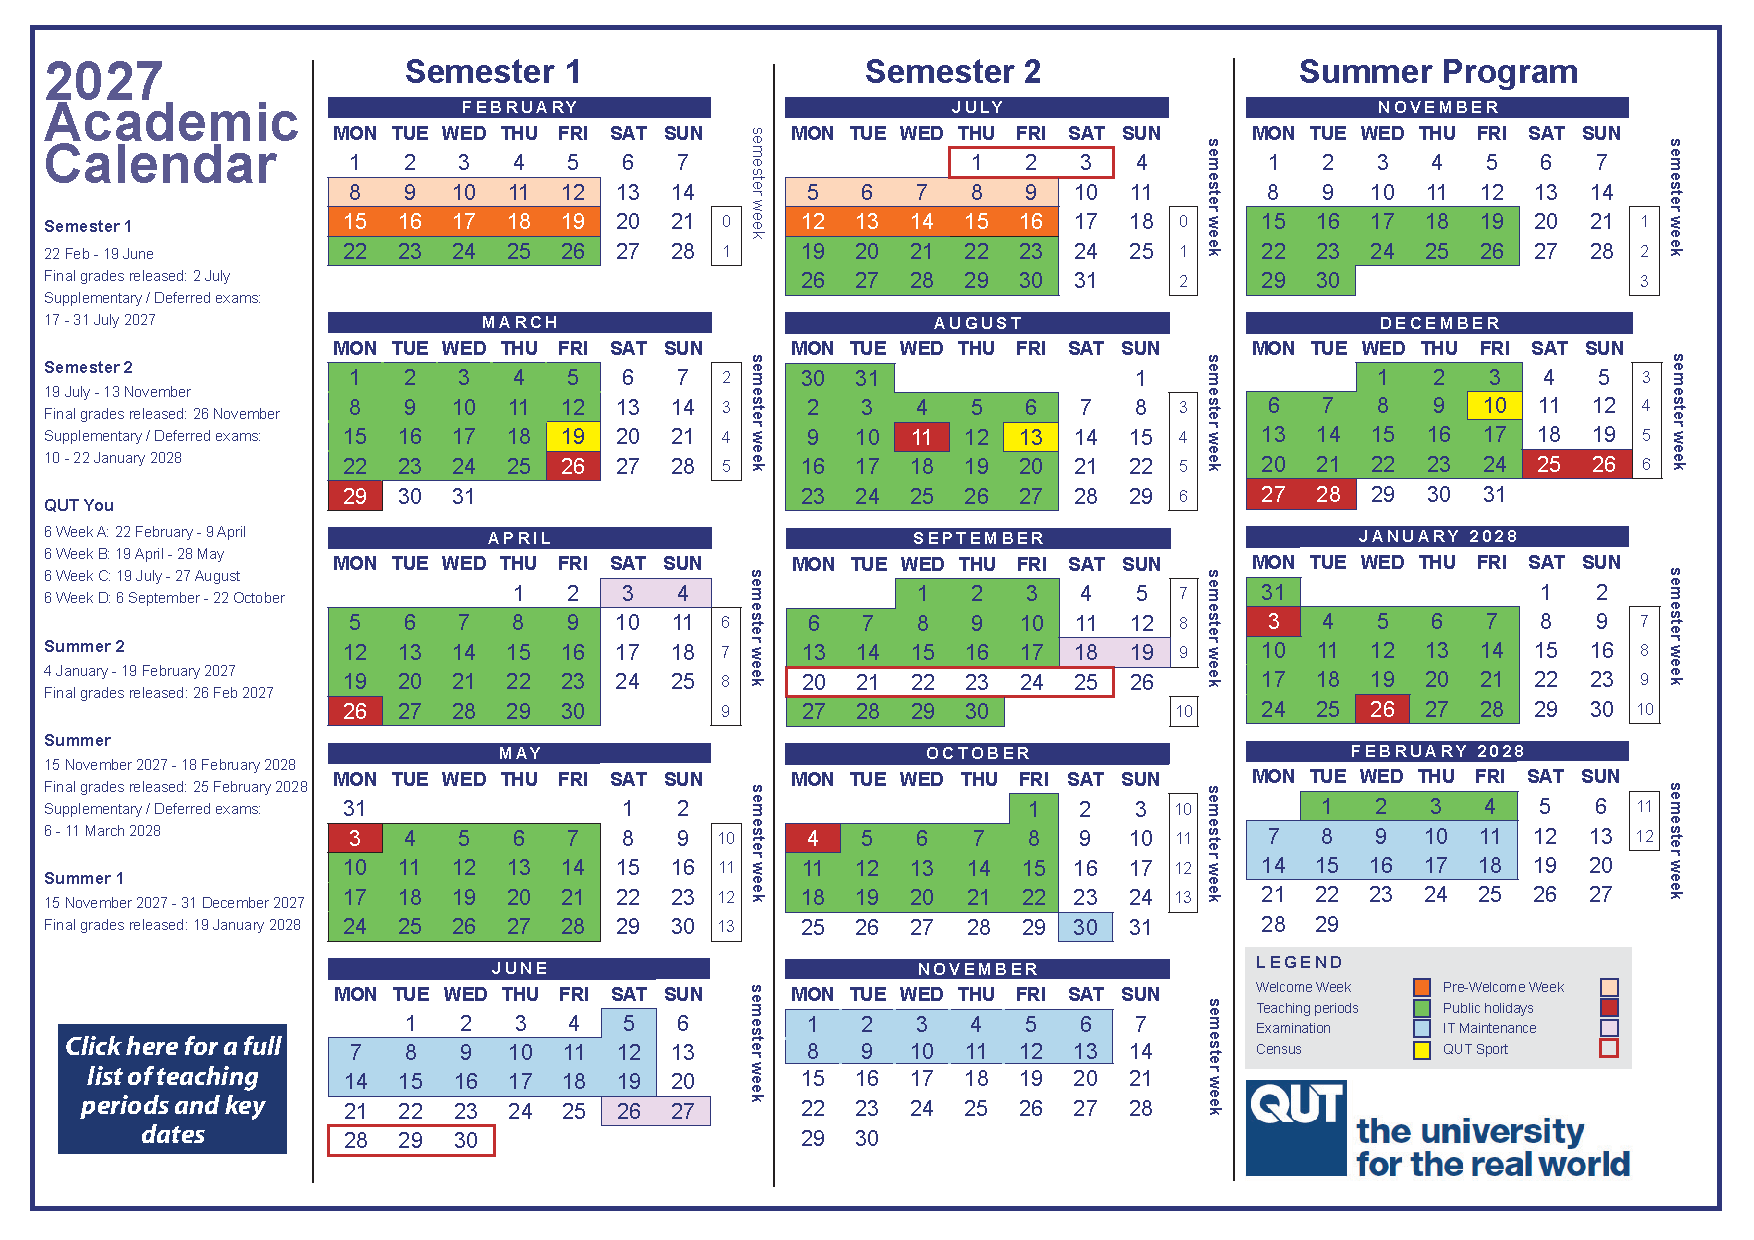
\includegraphics{pics/qut-academic-calendar-2027.pdf}}
\setlength{\qutcalendarwidth}{\wd\qutcalendarbox}
\setlength{\qutcalendarheight}{\dimexpr\ht\qutcalendarbox+\dp\qutcalendarbox\relax}
\paperwidth=\qutcalendarwidth
\paperheight=\dimexpr\qutcalendarheight+55mm\relax
\pagewidth=\qutcalendarwidth
\pageheight=\dimexpr\qutcalendarheight+55mm\relax
\newgeometry{margin=0mm}
\thispagestyle{empty}
\refstepcounter{section}
\label{app:qut-calendar}
\addcontentsline{toc}{section}{\protect\numberline{\thesection}QUT 2027年学术日历}

\begin{minipage}{\qutcalendarwidth}
  \vspace*{5mm}
  {\scriptsize\hbox to \qutcalendarwidth{\hspace*{25mm}\thesection\quad QUT 2027年学术日历\hfil\thepage\hspace*{25mm}}\par}
  \vspace{3mm}
  \begin{minipage}{\dimexpr\qutcalendarwidth-50mm\relax}
    \centering
    {\large\bfseries \thesection\quad QUT 2027年学术日历\par}
    \vspace{2mm}
    {\small 来源：\official{https://www.qut.edu.au/about/key-dates-and-academic-calendar/academic-calendar/2027-academic-calendar}{QUT 2027 Academic Calendar 官方页面}\par}
    \vspace{1.5mm}
    \raggedright
    {\footnotesize 以下为 QUT 官方发布的 2027 Academic Calendar, 包含 Semester 1, Semester 2, QUT You, Summer 和考试安排. PS: QUT You 是给 QUT 大一新生上的公共课, 我们不需要学习.\par}
  \end{minipage}
  \vspace{4mm}
\end{minipage}

\noindent\usebox{\qutcalendarbox}
\vspace*{7mm}
\clearpage
\restoregeometry
\paperwidth=210mm
\paperheight=297mm
\pagewidth=210mm
\pageheight=297mm

\clearpage
\qutmapsection{app:geography}{昆士兰州与布里斯班地理信息}
\qutmapappendixpage
  {\official{https://www.worldmap1.com/map-australia.asp}{WorldMap1 -- Map Australia}}
  {昆士兰州简称昆州. 下面按“澳大利亚--昆士兰州--布里斯班”的顺序递进展示位置关系. 澳大利亚各州及领地示意图.}
  {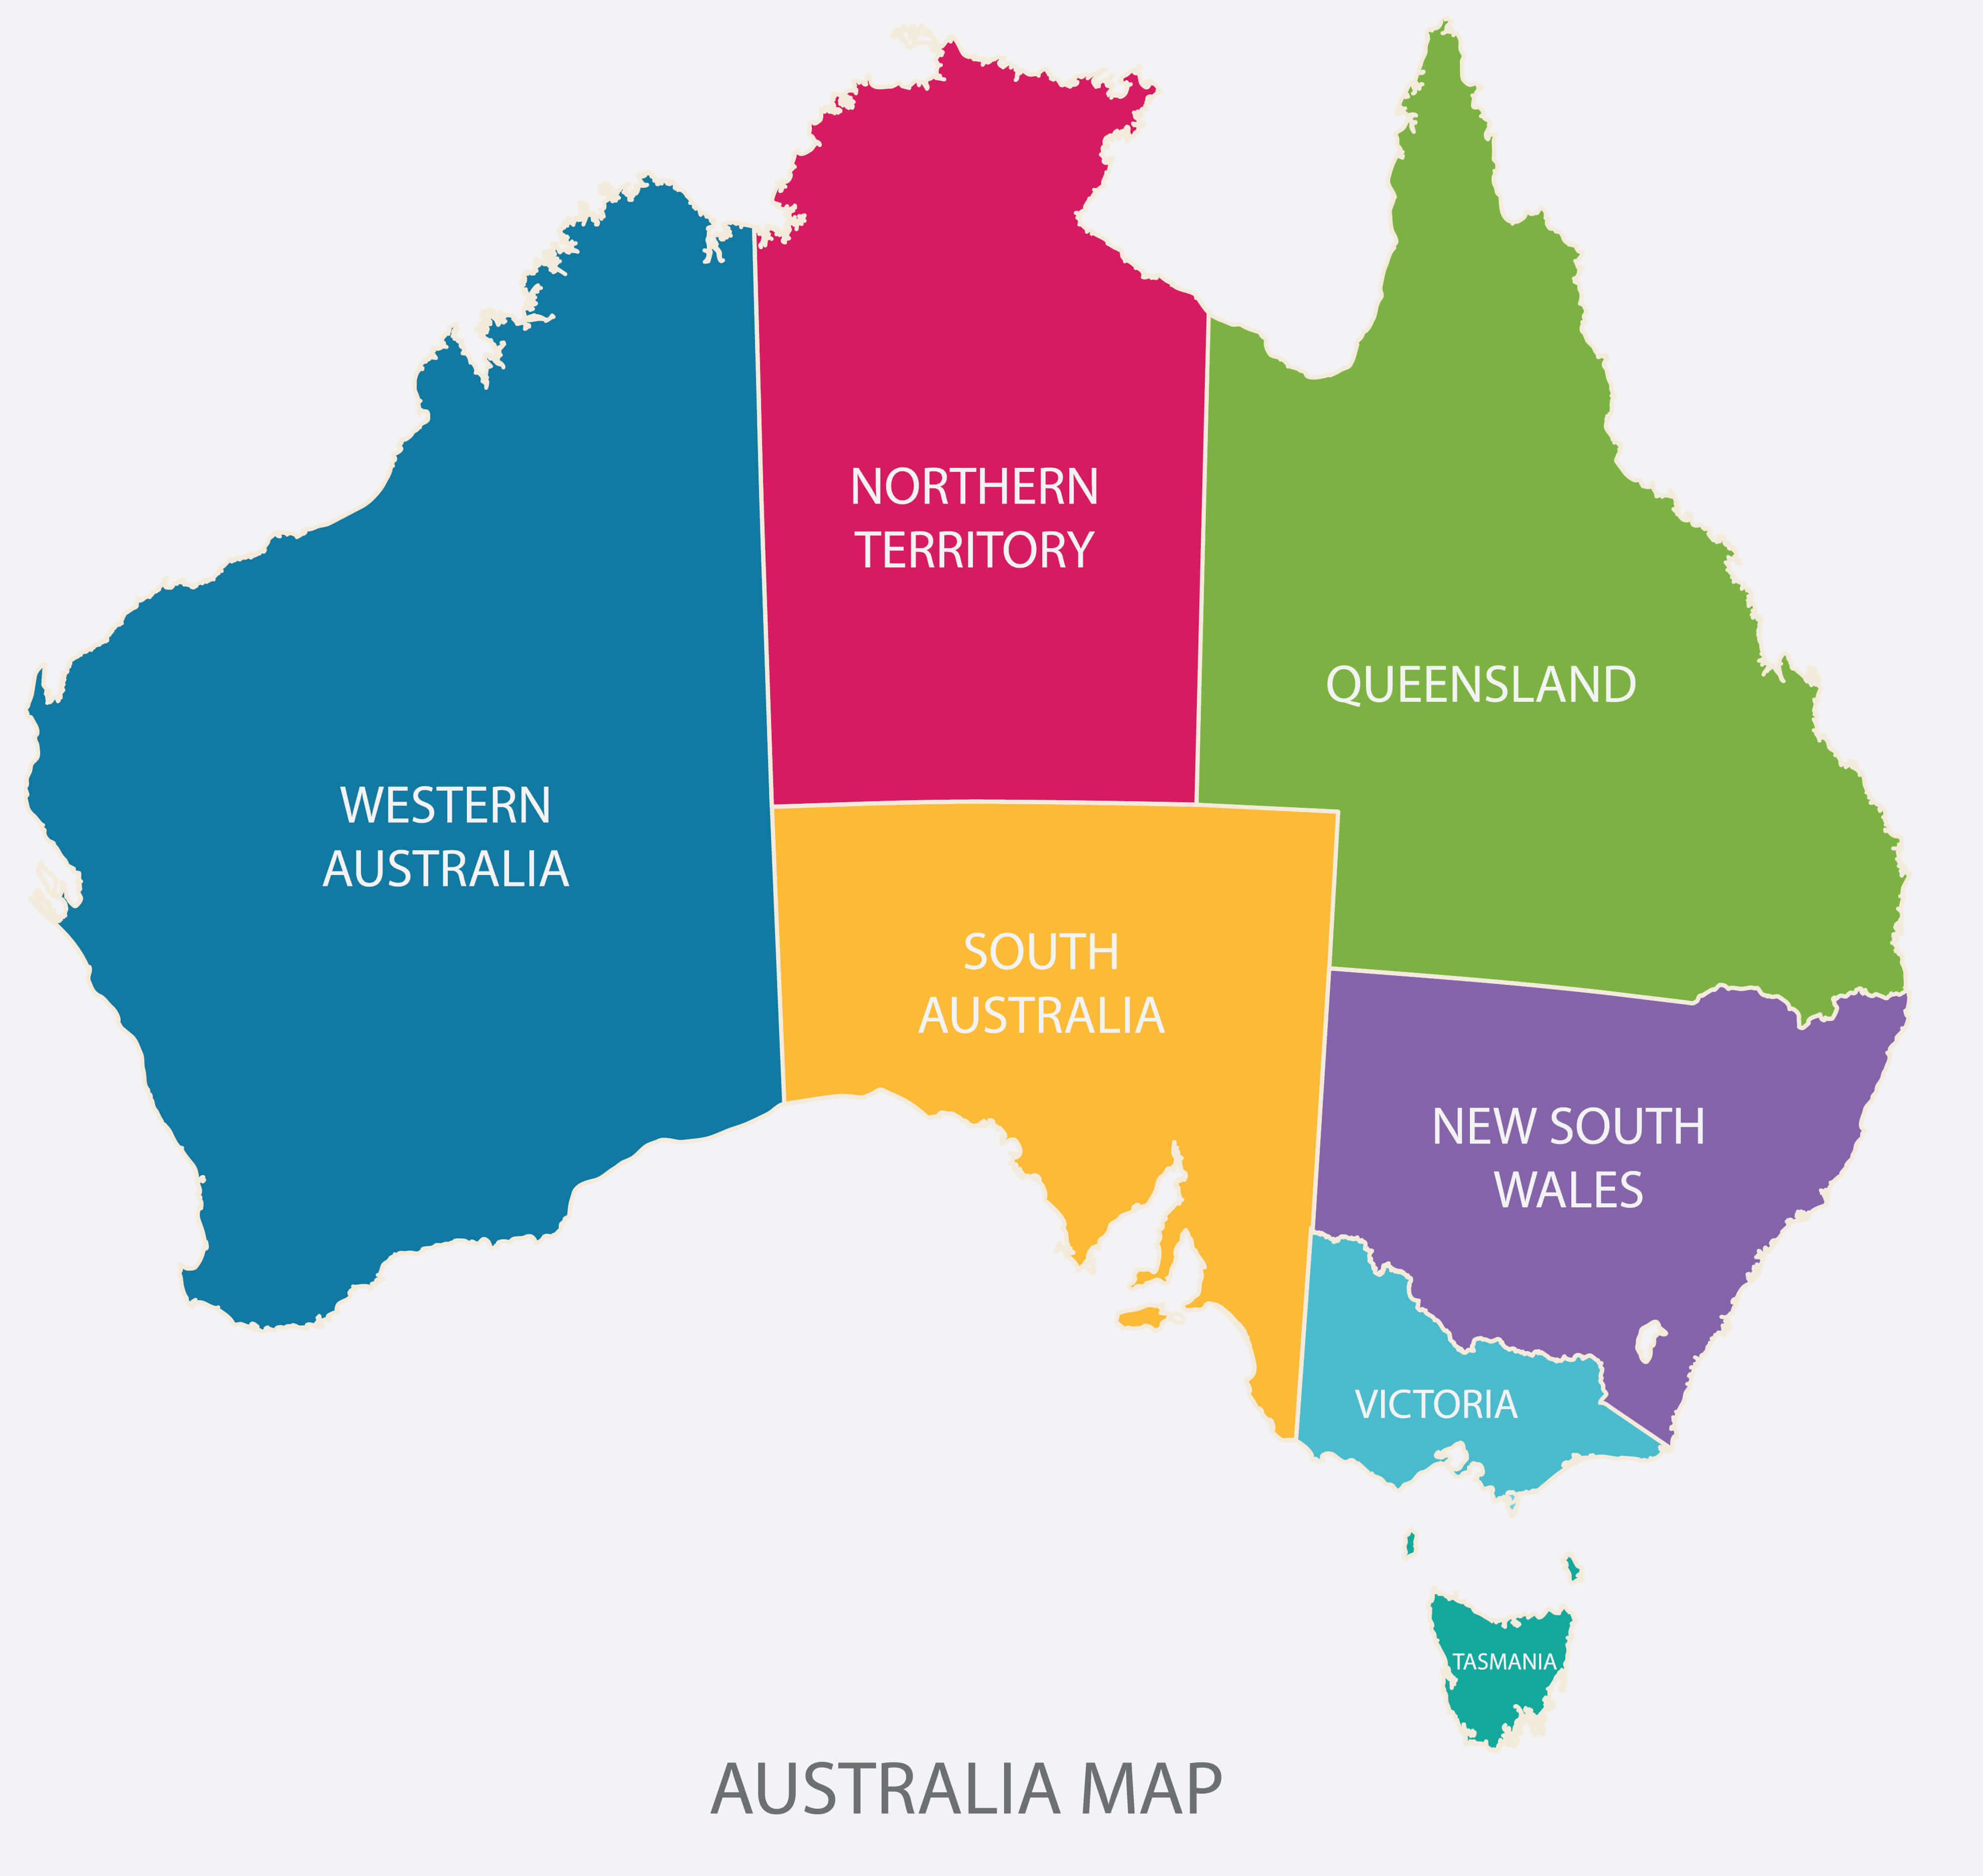
\includegraphics[width=\textwidth]{pics/aus-map.jpg}}
\qutmapappendixpage
  {\official{https://www.mapnations.com/countries/australia/states/queensland-map.html}{MapNations -- Queensland Map}}
  {昆士兰州行政区地图.}
  {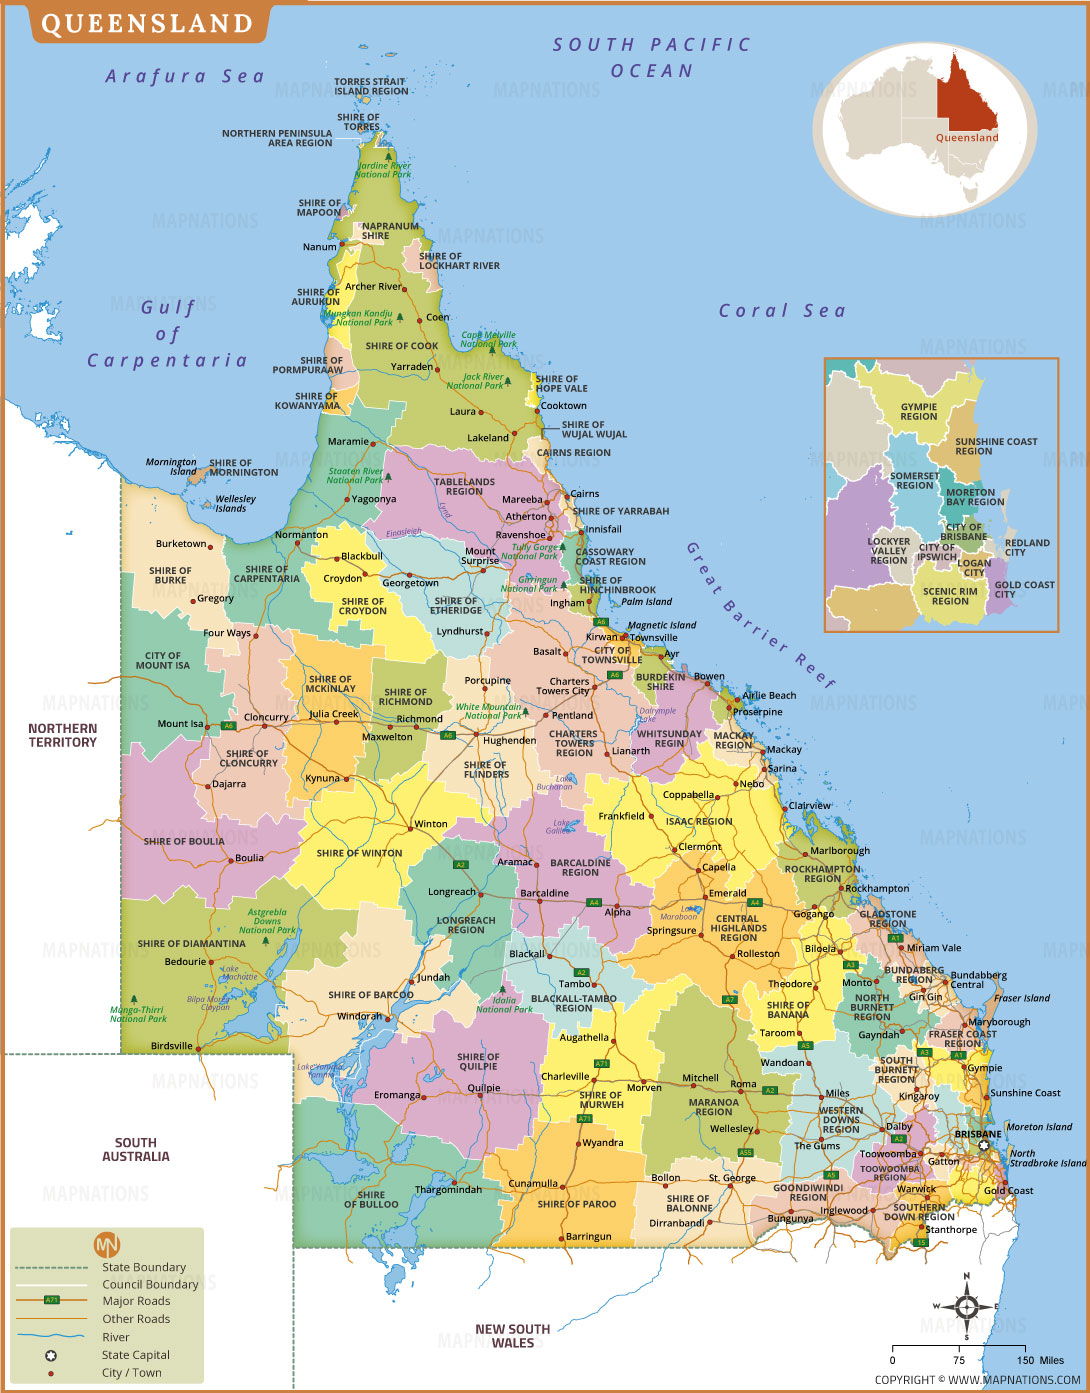
\includegraphics[width=\textwidth]{pics/queensland-map.jpg}}
\qutmapappendixpage
  {\official{https://thingstodoinbrisbanemap.com.au/}{Things to Do in Brisbane Map}}
  {布里斯班城市地图（Brisbane-map.pdf 第 2 页）.}
  {\includegraphics[page=2]{pics/Brisbane-map.pdf}}

\qutmapsection{app:QUT-map}{QUT 相关的地图}
\qutmapappendixpage
  {\official{https://oceania.aib.world/wp-content/uploads/sites/10/2022/08/QUT-Brisbane-Maps.pdf}{QUT Brisbane Maps}}
  {Oceania 相关的 QUT 地图, 第 1 页.}
  {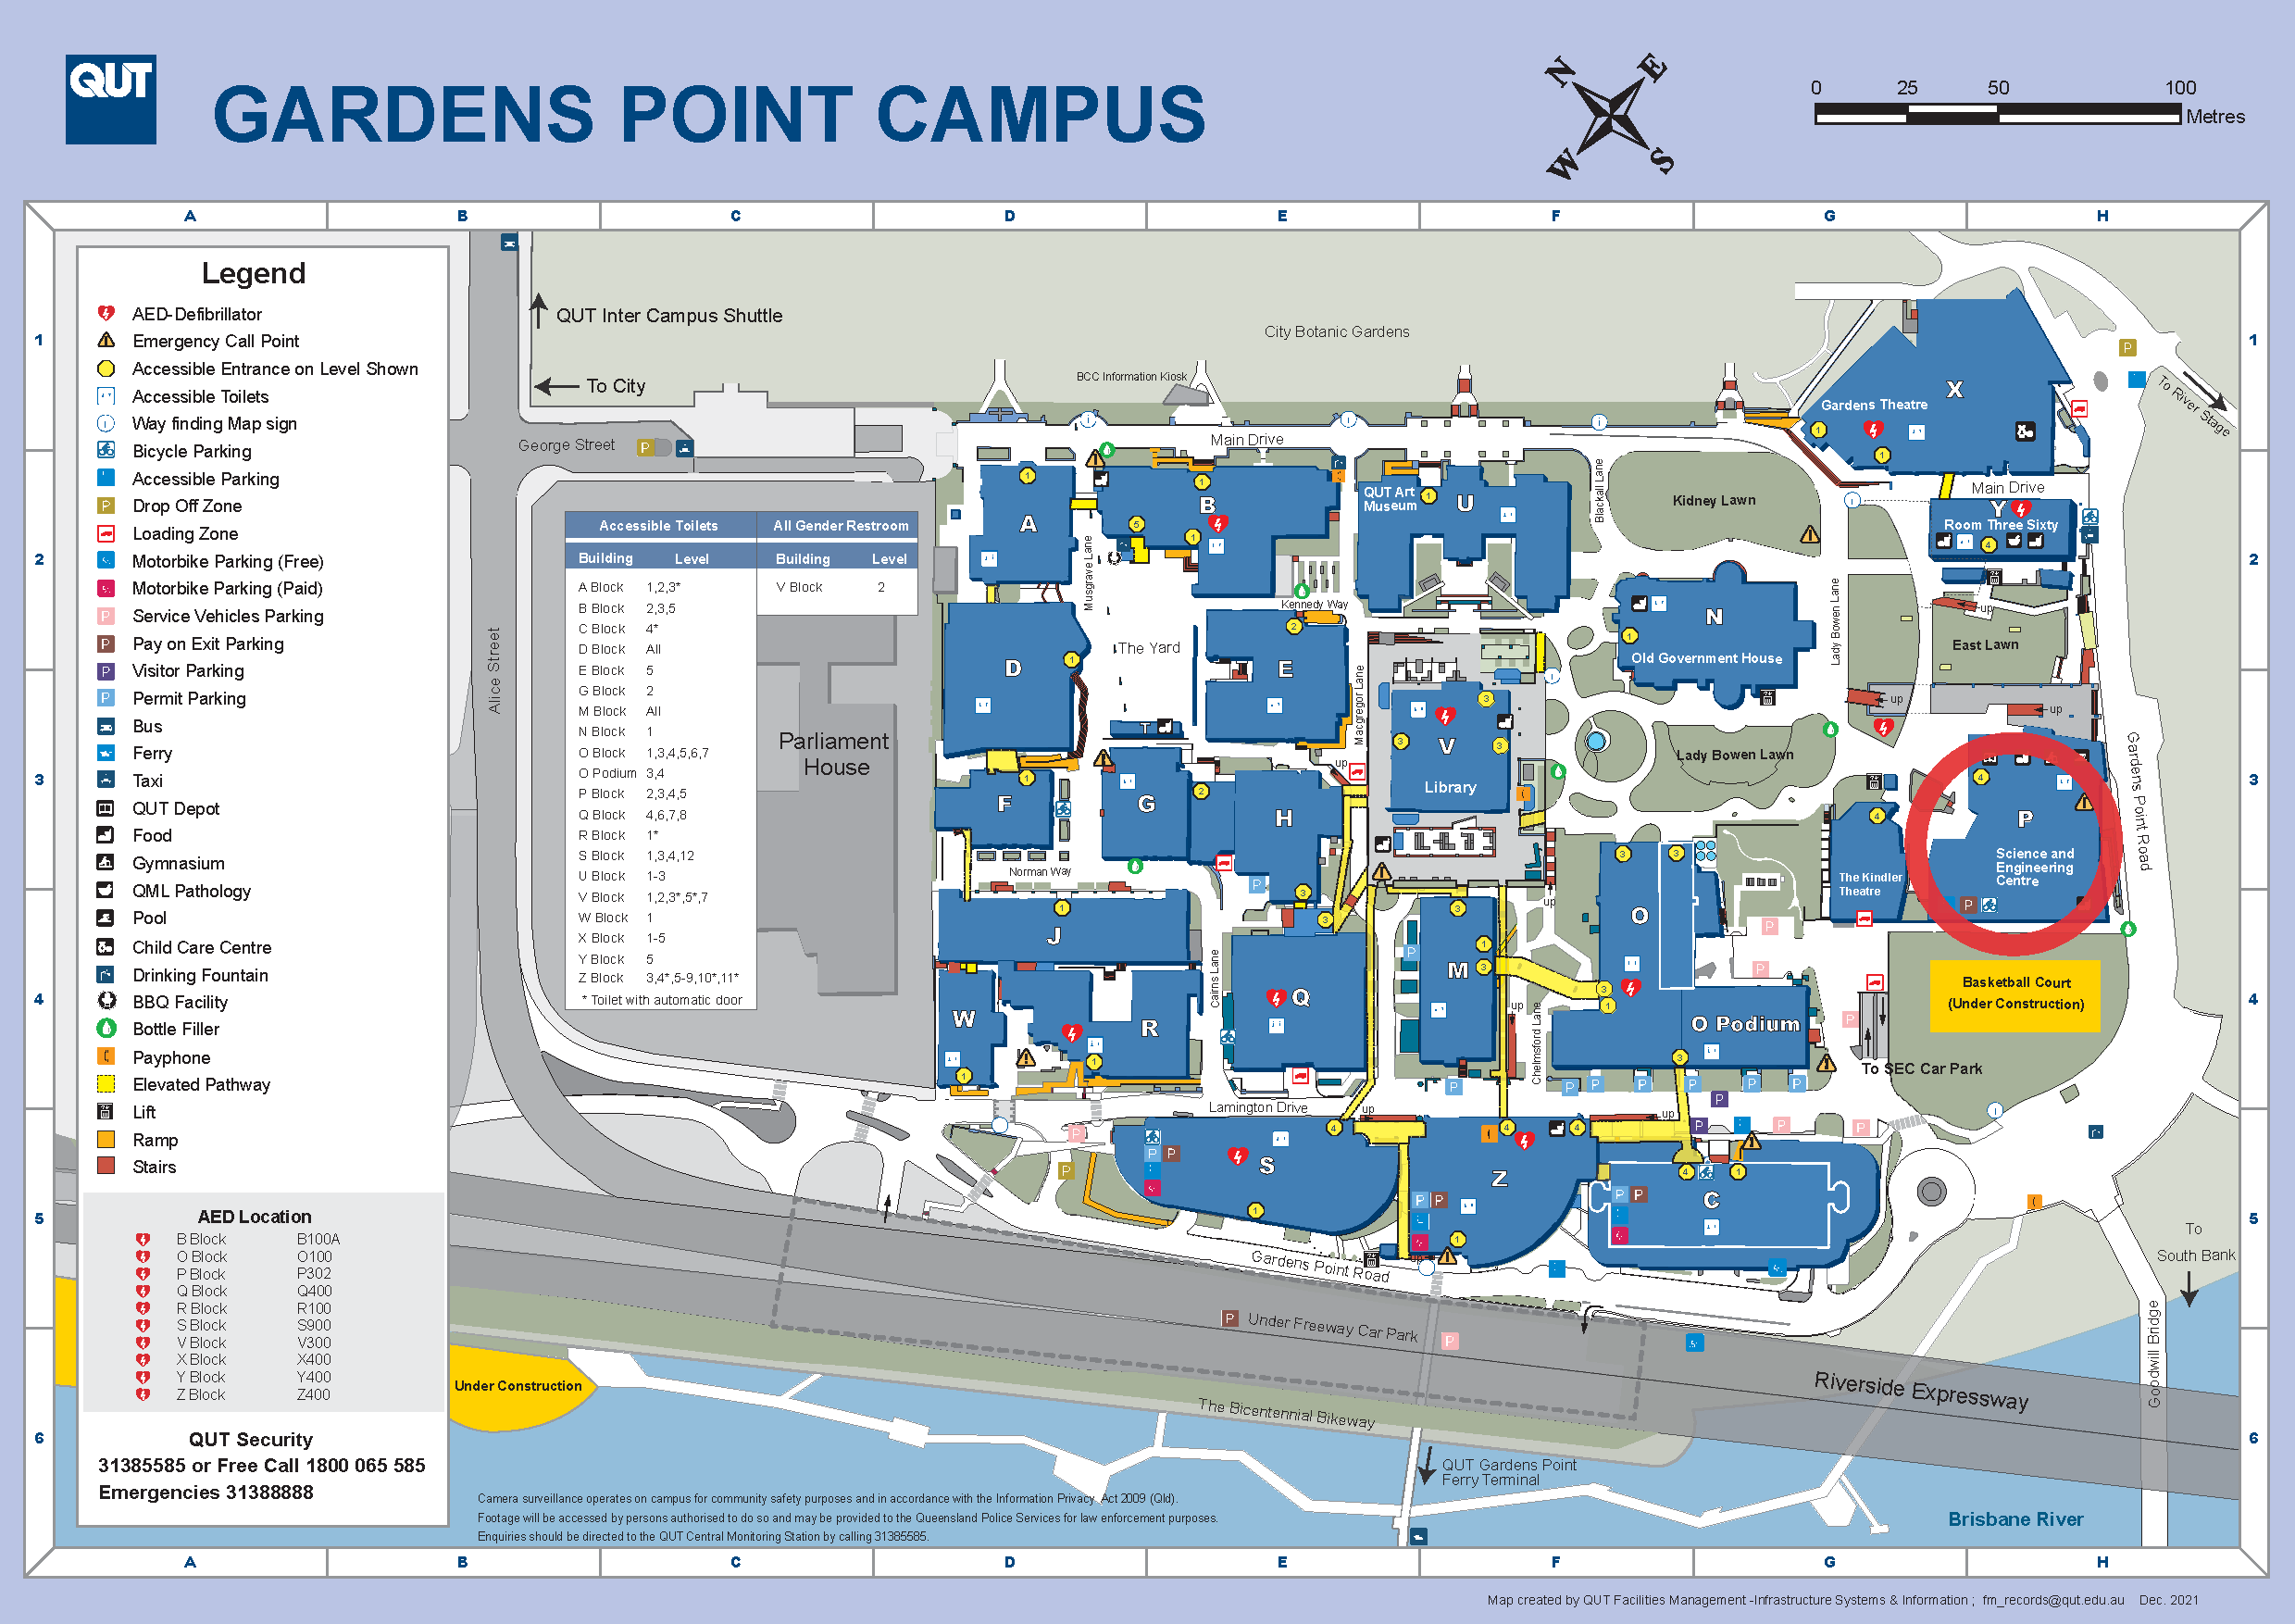
\includegraphics[page=1]{pics/QUT-Brisbane-Maps.pdf}}
\qutmapappendixpage
  {\official{https://oceania.aib.world/wp-content/uploads/sites/10/2022/08/QUT-Brisbane-Maps.pdf}{QUT Brisbane Maps}}
  {Oceania 相关的 QUT 地图, 第 2 页.}
  {\includegraphics[page=2]{pics/QUT-Brisbane-Maps.pdf}}
\qutmapappendixpage
  {\official{https://oceania.aib.world/wp-content/uploads/sites/10/2022/08/QUT-Brisbane-Maps.pdf}{QUT Brisbane Maps}}
  {Oceania 相关的 QUT 地图, 第 3 页.}
  {\includegraphics[page=3]{pics/QUT-Brisbane-Maps.pdf}}

\qutmapsection{app:jit-map}{金陵科技学院 (江宁校区) 地图}
\qutmapappendixpage
  {金陵科技学院 (江宁校区) 地图, 作者: 李京儒}
  {金陵科技学院 (江宁校区) 地图.}
  {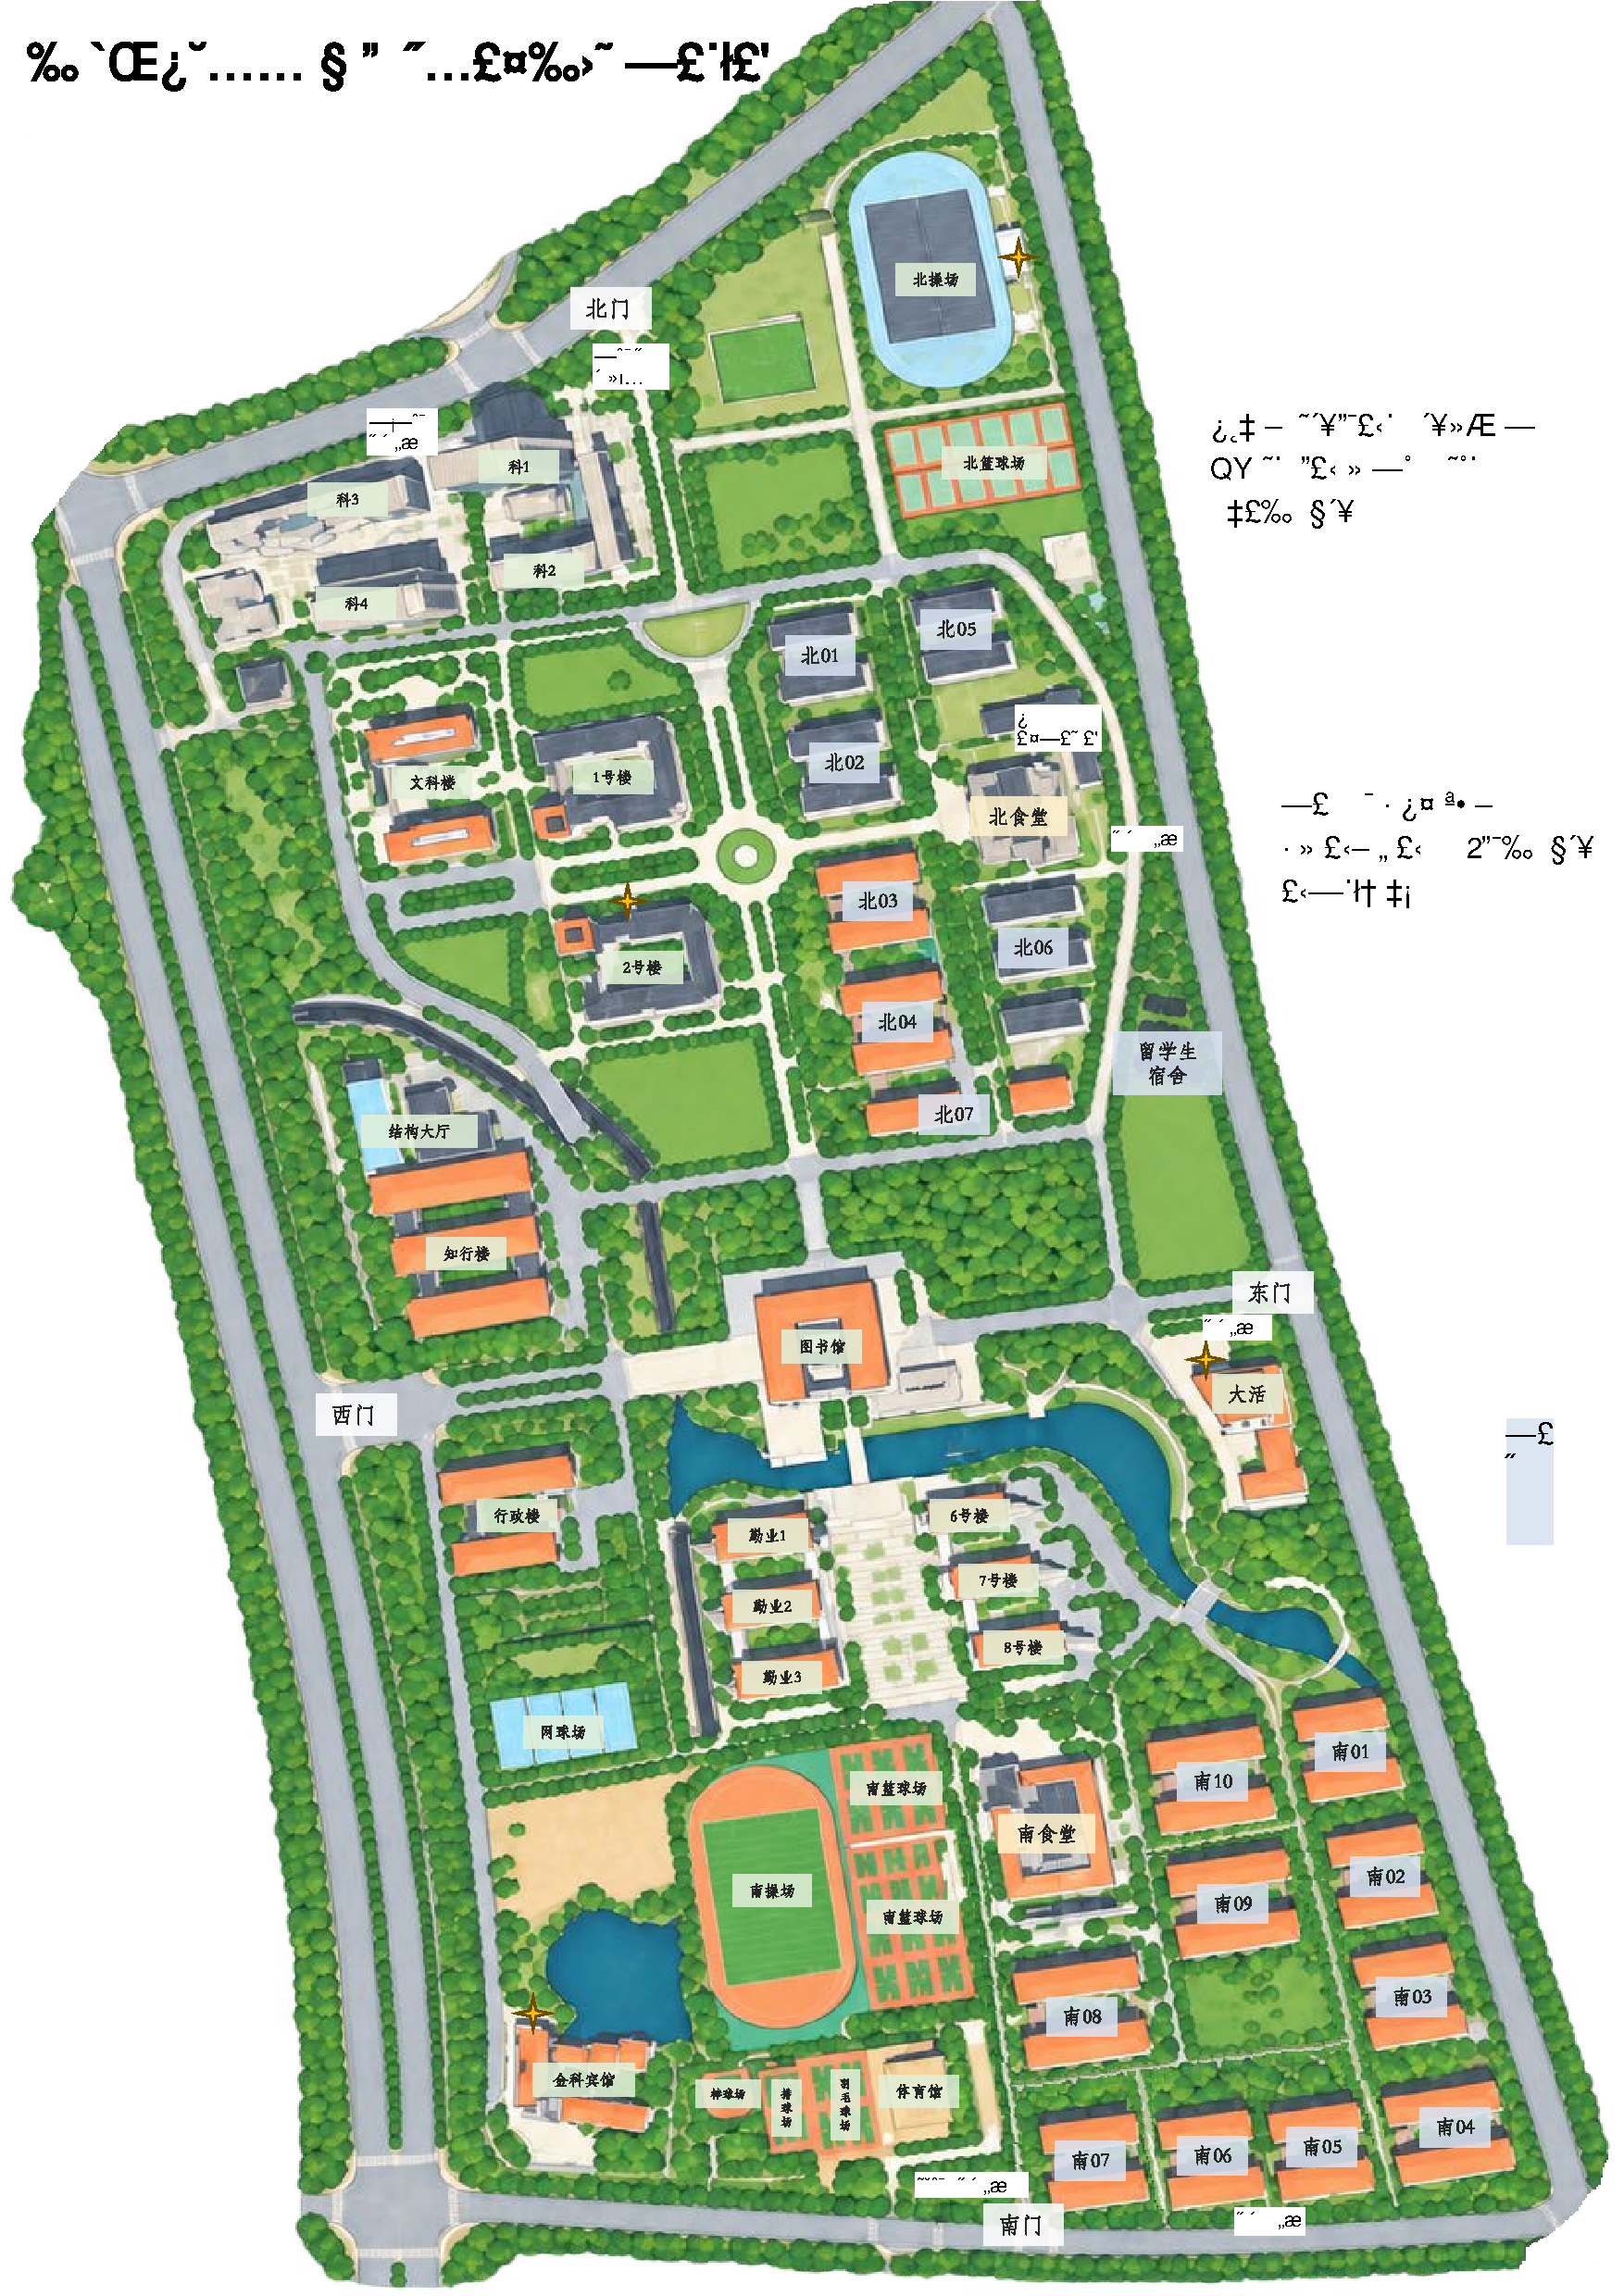
\includegraphics[page=1]{pics/map.pdf}}
\clearpage
\section{未达到语言要求时的语言班说明}\label{app:ielts-requirement}

下表将 2026 年语言入学要求整理为文字表格, 便于和自己的 IELTS, PTE 或 TOEFL 成绩对照. 语言班和主课入学要求可能调整, 实际申请时应以 QUT 官方语言要求, QUT College 课程安排以及个人 offer 为准.

\begin{center}
\textbf{\textcolor{red}{QUT 昆士兰科技大学 2026 年语言入学要求}}
\end{center}

\begingroup
\small
\setlength{\parindent}{0pt}
\setlength{\parskip}{0.58em}

\textbf{直接入读主专业: }2026 年 7 月入学

\textbf{雅思要求 (接受单项重考): }总分 6.5, 单项 6.0

\textbf{PTE 要求: }总分 58, 单项 50

\textbf{托福要求: }总分 79, 听力/阅读 16, 写作 21, 口语 18

\vspace{0.75em}

\textbf{EAP2 标准课程 (10 周): }2026 年 11 月入学

\textbf{雅思要求 (接受单项重考): }总分 6.0, 阅读/写作 5.5, 听力/口语 5.0

\textbf{PTE 要求: }总分 50, 听力/口语 38, 阅读/写作 46

\textbf{托福要求: }总分 71, 听力 10, 阅读/口语 14, 写作 18

\vspace{0.75em}

\textbf{EAP2 加长课程 (15 周): }2026 年 10 月入学

\textbf{雅思要求 (接受单项重考): }总分 5.5, 阅读/写作 5.5

\textbf{PTE 要求: }总分 46, 阅读/写作 46

\textbf{托福要求: }总分 56, 阅读 14, 写作 18

\vspace{0.75em}

\textbf{EAP1 标准课程 (20 周): }2026 年 11 月入学

\textbf{雅思要求 (接受单项重考): }总分 5.0, 阅读/写作 5.0, 听力/口语 4.5

\textbf{PTE 要求: }总分 46, 听力/口语 32, 阅读/写作 38

\textbf{托福要求: }总分 56, 听力/阅读 8, 写作 15, 口语 12

\vspace{0.75em}

\textbf{EAP1 加长课程 (25 周): }2026 年 10 月入学

\textbf{雅思要求 (接受单项重考): }总分 5.0, 阅读/写作 5.0

\textbf{PTE 要求: }总分 38, 阅读/写作 38

\textbf{托福要求: }总分 49, 阅读 10, 写作 15

\endgroup

\clearpage
\section{校园跑细则}\label{app:school-running}

\begin{figure}[H]
	\centering
	{\small 来源: 金陵科技学院校园跑细则文件\par\vspace{0.6em}}
	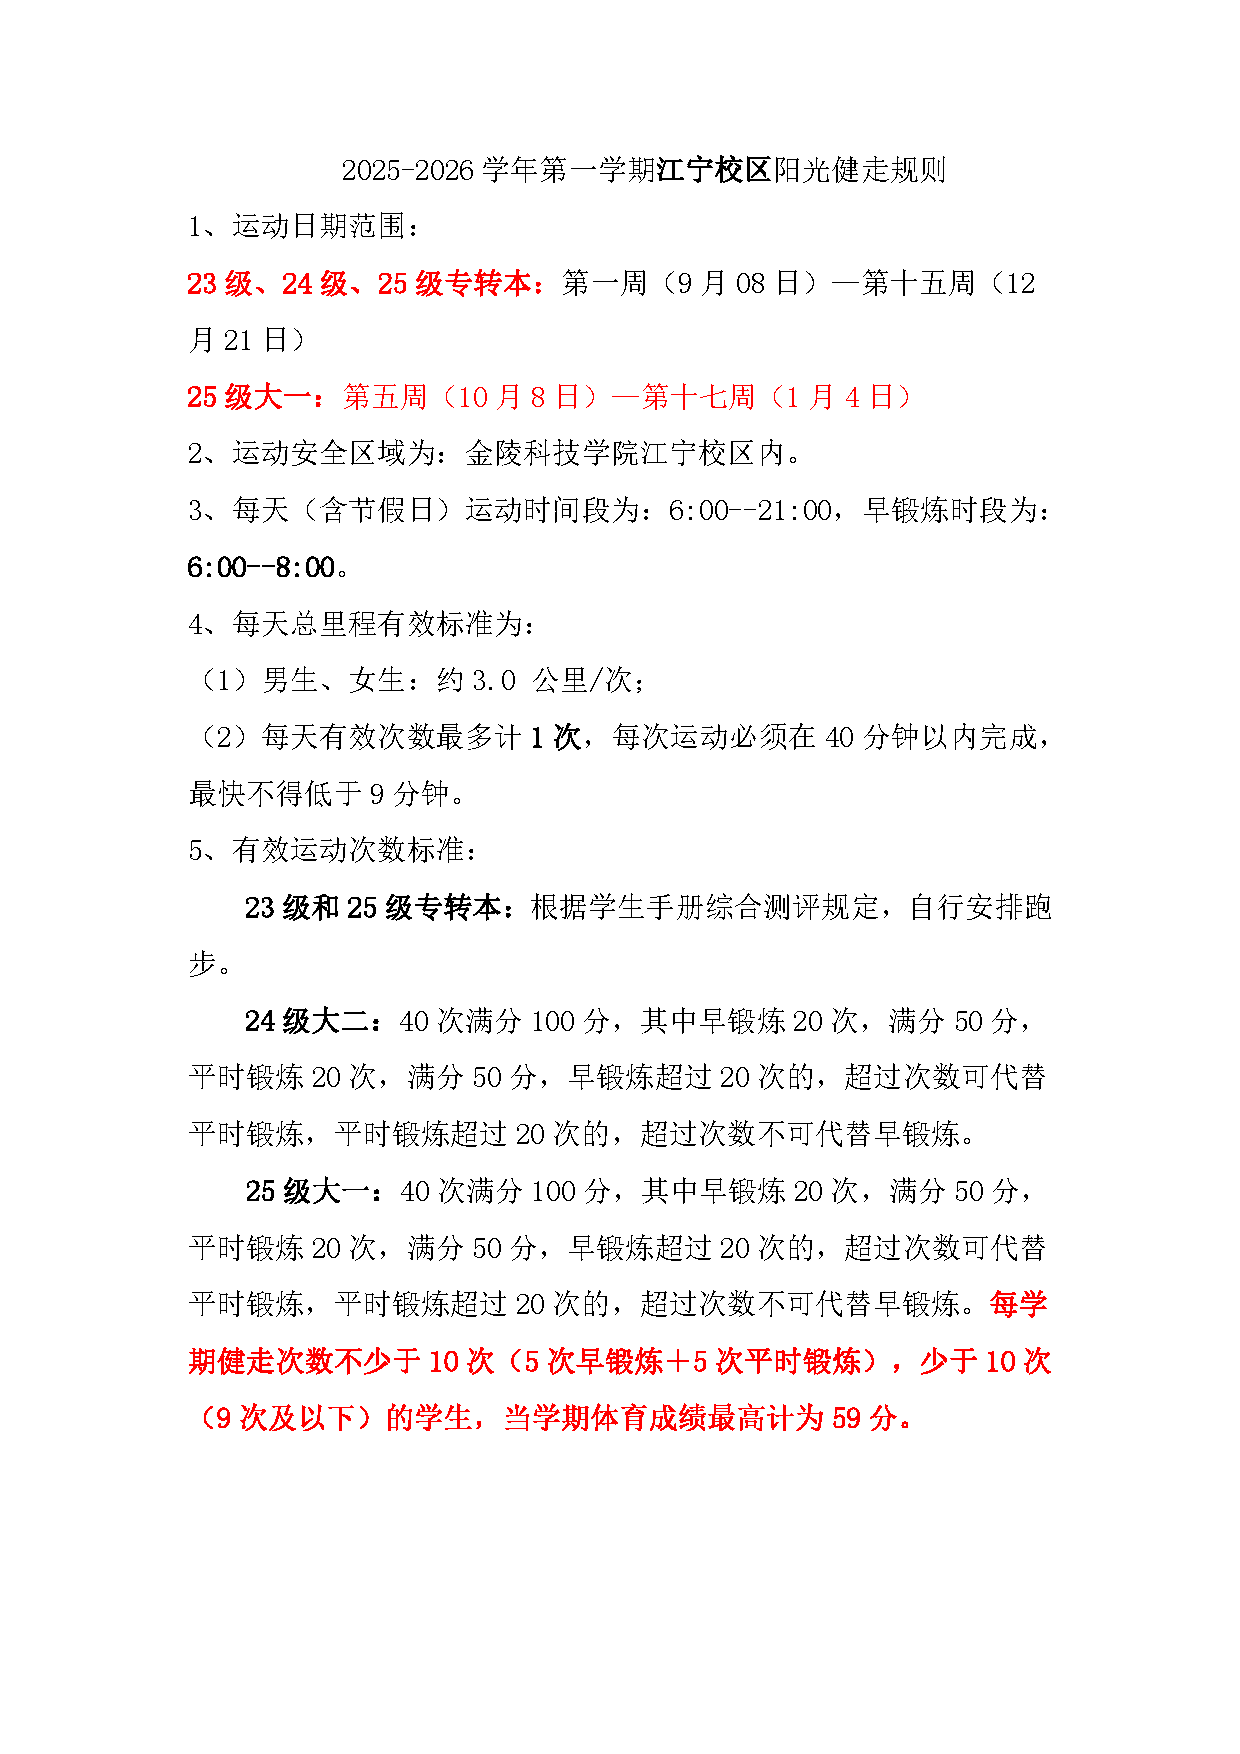
\includegraphics[page=1,width=1\textwidth,keepaspectratio]{pics/school-running.pdf}
\end{figure}
\clearpage
\begin{figure}[H]
	\centering
	{\small 来源: 金陵科技学院校园跑细则文件\par\vspace{0.6em}}
	\includegraphics[page=2,width=1\textwidth,keepaspectratio]{pics/school-running.pdf}
\end{figure}
\clearpage
\begin{figure}[H]
	\centering
	{\small 来源: 金陵科技学院校园跑细则文件\par\vspace{0.6em}}
	\includegraphics[page=3,width=1\textwidth,keepaspectratio]{pics/school-running.pdf}
\end{figure}

\clearpage
\section{澳洲房型介绍}\label{app:room}

\begin{figure}[H]
  \centering
  \begin{minipage}[t]{0.48\textwidth}
    \centering
    \includegraphics[width=\linewidth]{pics/room\_1.jpg}
    \par\smallskip
    {\small 来源：异乡好居\par}
  \end{minipage}\hfill
  \begin{minipage}[t]{0.48\textwidth}
    \centering
    \includegraphics[width=\linewidth]{pics/room\_2.jpg}
    \par\smallskip
    {\small 来源：异乡好居\par}
  \end{minipage}
\end{figure}





\end{document}
